% Paper v9 -- popular companion (EN), 2026-05-06.
% Companion to the formal paper paper_v9_en.tex; all factual claims,
% empirical numbers, tables, and conclusions are taken from v9 main,
% only the tone is translated into language accessible to a technically
% curious layperson or crypto-curious developer (knows hash and AES,
% does not know DLP/lattice/formal cryptography).
%
% v9 SCOPE CORRECTION: Grata Cascade reframed as one-shot KE primitive
% (NOT CKA). Changes vs pop v8:
% - title: subtitle updated to v9
% - §1.3 hook: "fourth ratchet" → "third independent assumption for hybrid
%   post-quantum key establishment" (X-Wing hook)
% - §8 comparison: ECDH, ML-KEM, X-Wing, Merkle puzzles (NOT Triple Ratchet)
% - §9 added prob:cka-extension as primary follow-up direction
% - §10 conclusion: positioning as "third coequal layer in X-Wing hybrid",
%   not "fourth ratchet"
% - minor wording updates in §3-§7 (CKA → key agreement)
%
% Reference v2 (canonical): L=32, N=4096, h_AB=5, h_BA=2, h_P=8, M=8,
% s=4, p_upd=0.75, lambda=120 bits. v3 candidate: reference_h_AB6.
% Empirical numbers identical to paper_v9_en.tex (50k convergence,
% 99.9920% KM, NIST 12/12 PASS, 0/300 attackers).
%
% Source of truth for all numbers: paper_v9_en.tex + docs/glossary.md.
% Editing the popular version requires keeping consistency with main paper.

\documentclass[11pt,a4paper]{article}
\usepackage[utf8]{inputenc}
\usepackage[T1]{fontenc}
\usepackage{amsmath,amssymb}
\usepackage{geometry}
\usepackage{hyperref}
\usepackage{url}
\usepackage{booktabs}
\usepackage{enumitem}
\usepackage{xcolor}
\usepackage{tikz}
\usepackage[most]{tcolorbox}

\usetikzlibrary{positioning,arrows.meta,shapes.geometric,fit,backgrounds,calc}

\geometry{margin=2.5cm}

\hypersetup{
    colorlinks=true,
    linkcolor=black,
    urlcolor=blue,
    citecolor=black
}

% --- Popular boxes: TL;DR, Aha moment, Sidebar, Warning ---

\definecolor{tldrbg}{RGB}{235,242,255}
\definecolor{tldrframe}{RGB}{30,80,160}
\definecolor{ahabg}{RGB}{255,247,225}
\definecolor{ahaframe}{RGB}{180,120,20}
\definecolor{sidebarbg}{RGB}{240,240,240}
\definecolor{sidebarframe}{RGB}{100,100,100}
\definecolor{warnbg}{RGB}{255,235,235}
\definecolor{warnframe}{RGB}{180,40,40}

\newtcolorbox{tldr}[1][TL;DR]{
  colback=tldrbg, colframe=tldrframe,
  fonttitle=\bfseries, title={#1},
  boxrule=0.6pt, arc=2pt, left=8pt, right=8pt, top=6pt, bottom=6pt,
  breakable
}

\newtcolorbox{aha}[1][Aha moment]{
  colback=ahabg, colframe=ahaframe,
  fonttitle=\bfseries, title={#1},
  boxrule=0.6pt, arc=2pt, left=8pt, right=8pt, top=6pt, bottom=6pt,
  breakable
}

\newtcolorbox{sidebar}[1][For the mathematically curious]{
  colback=sidebarbg, colframe=sidebarframe,
  fonttitle=\bfseries\itshape, title={#1},
  boxrule=0.4pt, arc=2pt, left=8pt, right=8pt, top=6pt, bottom=6pt,
  breakable
}

\newtcolorbox{warning}[1][Warning]{
  colback=warnbg, colframe=warnframe,
  fonttitle=\bfseries, title={#1},
  boxrule=0.6pt, arc=2pt, left=8pt, right=8pt, top=6pt, bottom=6pt,
  breakable
}

\title{Grata Cascade: An Accessible Companion\\
\large Popular companion to paper v9}

\author{Robert Jarušek\\Grata Luma s.r.o., Prague}
\date{}

\begin{document}

\maketitle

\begin{tldr}[What this booklet is]
This is a \emph{popular companion} to the formal paper \emph{Grata Cascade: Hash-based One-Shot Key Agreement via Statistical Drift, as a Candidate for Hybrid Post-Quantum Key Establishment} (v9). It contains the same factual content --- all claims, empirical numbers, tables, and conclusions --- but written in language accessible to anyone who knows what a hash function and a cipher are. For full mathematics, proofs, and citations we point to the main paper. The goal: an amateur should be able to understand the protocol.
\end{tldr}

\medskip
\noindent\emph{Birthday paradox describes a static state. Grata Cascade builds a dynamic one-shot system on top of it. The continuous (CKA) variant remains open.}

\tableofcontents
\bigskip

\section{Introduction: A Game with Three Numbers}\label{pop:intro}

\subsection{A toy game to fix intuition}

Imagine a simple game. Three people --- Alice, Bob, and the eavesdropper Eve --- sit in separate rooms. Each is given the same board with numbers 1 through 10 and independently picks three of them. Alice and Bob want to agree publicly (over a channel that Eve listens in on) on some number that \emph{both of them independently picked}. Eve wants to guess that number.

Two questions follow.

\paragraph{Question 1.} \emph{What is the probability that Alice and Bob picked at least one number in common?} Combinatorics gives the answer: out of 10 numbers Bob picks 3, and the chance that none of his picks are in Alice's three is $\binom{7}{3}/\binom{10}{3} = 35/120 \approx 29\%$. So the probability that the intersection is non-empty is roughly \textbf{71 \%}. A solid chance --- in the vast majority of cases Alice and Bob have something to share.

\paragraph{Question 2.} \emph{Eve also picks three numbers. What is the probability that Eve's three contain a number that Alice and Bob agreed on?} For Eve to succeed, one of her three picks has to be simultaneously in Alice's three and in Bob's three (i.e.\ in $A \cap B$). This is the classic \emph{three-way birthday problem} and the answer is roughly \textbf{26 \%}.

See the gap? Alice and Bob agree in 71 \% of cases. Eve, despite using exactly the same "computational resources" (she also picks three numbers from ten), hits their agreement only 26 \% of the time. The ratio 71/26 $\approx$ \textbf{2{,}7}. Eve is structurally at a disadvantage even though she is playing exactly the same game.

\begin{aha}[Structural asymmetry]
Eve has less information than Alice and Bob, and no amount of computation will help her close the gap. This inequality is not computational; it is a property of the \emph{geometry of the problem}: a two-way intersection ($A \cap B$) is always larger than a three-way one ($A \cap B \cap E$). Even with unlimited time and a quantum computer, Eve stays in the 26 \% regime.
\end{aha}

For our toy game with ten numbers the gap is only 2{,}7$\times$. In real cryptography we will be using a space of size $2^{256}$ instead of ten and each party picks $k = 4096$ vectors instead of three. The asymmetry ratio is then no longer 2{,}7$\times$ but $\approx 2^{244}$ --- astronomical. We work this out in detail in Chapter~\ref{pop:static}.

\subsection{From toy to cryptography}

The game with ten numbers is, of course, a toy. Real cryptography works with a space of size $2^{256}$ (32-byte vectors, so $256^{32} = 2^{256}$ possible values --- a number with 78 decimal digits) instead of ten. But the principle remains: if we can find a way for Alice and Bob to \emph{communicate publicly} --- without the public messages \emph{revealing} which intersection element they found --- we have the building block of a cryptographic protocol.

This is non-trivial because the communication has to do two things at once:
\begin{enumerate}[leftmargin=*]
\item Alice and Bob \emph{must} manage to agree on something (otherwise the game is pointless).
\item The public communication \emph{must not} betray what they agreed on (otherwise Eve wins).
\end{enumerate}

Grata Cascade is one answer: a parametric family of protocols that pulls this off. It is not the first such attempt --- there are protocols based on Diffie-Hellman (classical), on lattices (post-quantum ML-KEM), on hashes in Tree Parity Machine (historical). But Grata Cascade has one property that sets it apart: it rests solely on \emph{hash preimage resistance} and \emph{statistical drift of shared state}. No Diffie-Hellman. No lattices. Just hashes and shared information.

\subsection{Why should we care about a third independent assumption?}\label{pop:why-third-assumption}

\noindent\emph{A quick note on orientation.} The cryptographic literature talks a lot about \emph{ratchets} --- mechanisms that progressively rotate the key forward, never backward. They are useful for \emph{continuous} key agreement in messaging (Signal Triple Ratchet rotates the key between messages). \emph{This work is not building a ratchet} --- it is building something smaller: a one-shot key agreement primitive. Meaning ``Alice and Bob run the protocol, it terminates, they get one key, done.'' No ongoing rotation between messages. Extending it to a ratchet is a separate, open direction (see Chapter~\ref{pop:open}, \texttt{prob:cka-extension}). We mention ratchets here only to orient where Grata Cascade sits.

\medskip
When you write a message today (year 2026) over Signal or WhatsApp, the initial key agreement (before the ratchet kicks in) typically uses a \emph{hybrid KEM}: a combination of two one-shot primitives mixing classical and post-quantum cryptography. Concretely NIST recommends a scheme called \textbf{X-Wing} that combines:

\begin{itemize}[leftmargin=*]
\item \textbf{X25519} (elliptic-curve Diffie--Hellman) --- the classical layer. Vulnerable to Shor's algorithm on a quantum computer.
\item \textbf{ML-KEM-768} (lattice-based KEM, formerly Kyber) --- the post-quantum layer. Rests on the hardness of Module-LWE.
\end{itemize}

The adversary must break \emph{both} layers to recover the key. That is \emph{hybrid security} --- standard practice for the post-quantum era.

The open question that Grata Cascade addresses is: \emph{does there exist a third, practically usable one-shot primitive that stands on an entirely different principle than Diffie--Hellman or lattices?} If yes, the hybrid stack could carry three independent layers --- the adversary would have to simultaneously break DLP, lattices, \emph{and} that third assumption, which is structurally more robust than two pillars.

Grata Cascade is a candidate for that third layer. It does not rest on DH or on lattices; it rests purely on \emph{hash function preimage resistance} (a wholly different kind of assumption) combined with statistical drift. We will work through this gradually in the chapters ahead.

\subsection{What is proven and measured}

This subsection matters: \emph{before} we dive into details, let us put our cards on the table. After more than two years of development and empirical evaluation, what do we actually know?

\begin{tldr}[Empirical headline (reference v2, May 2026)]
\begin{itemize}[leftmargin=*]
\item \textbf{Convergence}: $50\,000$ runs, $100\%$ Final-hit, $99{,}9920\%$ keys-match. Upper bound (Clopper-Pearson, 95\% CI) on failure rate: $2{,}05 \times 10^{-4}$.
\item \textbf{Key randomness}: NIST SP 800-22 statistical battery, $12/12$ tests PASS over $1\,000$ keys.
\item \textbf{Adversary resilience}: 5 classes of passive adversaries (B.1-B.4, B.7), $0/300$ recoveries across all of them. Most sophisticated (B.4 AES-Oracle): Cohen's $d = 0{,}009$ --- no measurable discriminating power.
\item \textbf{H\_AB=6 ablation}: $0/50\,000$ divergences; CP upper bound $7{,}38 \times 10^{-5}$, below baseline. \texttt{reference\_h\_AB6} stands as a v3 reference candidate.
\item \textbf{Open}: formal reduction of dynamic asymmetry, ML adversaries, bandwidth optimisation, full evaluation on remaining profiles.
\end{itemize}
\end{tldr}

That is hard data. None of it is a theoretical estimate; every number comes from real protocol runs. We will walk through the evidence in Section~\ref{pop:empirical}, but if you only need one truthful summary: \emph{the protocol almost always converges, its output keys look like random noise, and not one of the five classified eavesdropping types reached the key.}

\subsection{Visualisation: same game, different outcomes}\label{pop:fig-asymmetry}

Figure~\ref{fig:asymmetry} shows why the "three out of ten" game gives the legitimate parties an edge. Left: Alice and Bob each independently pick three numbers, and in 71 \% of cases their intersection is non-empty (giving them something to agree on). Right: Eve also picks three numbers, but in only 26 \% of cases her three contain one of the numbers Alice and Bob picked in common.

\begin{figure}[h]
\centering
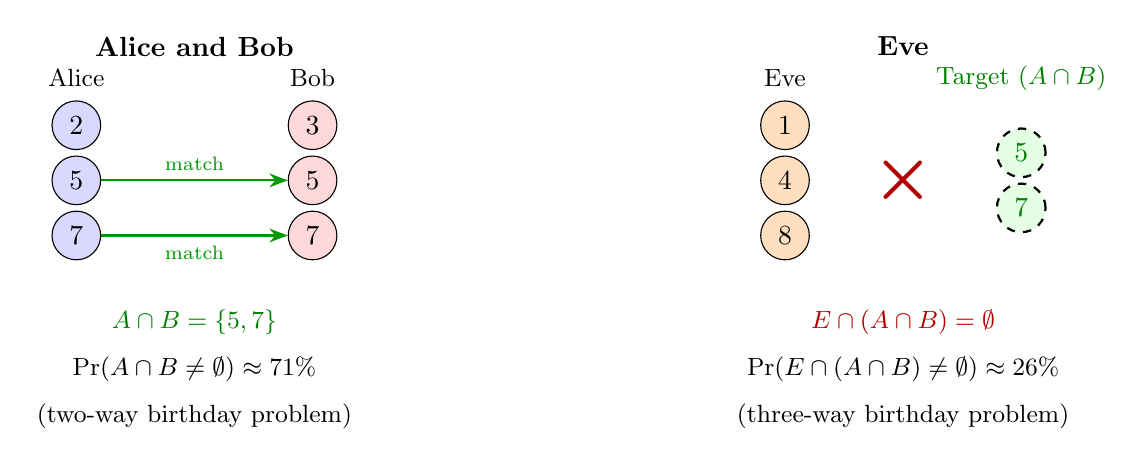
\begin{tikzpicture}[scale=1.0]
  % Left half: legitimate parties
  \begin{scope}[shift={(-4.5,0)}]
    \node[font=\bfseries] at (0, 2.4) {Alice and Bob};

    % Alice
    \node[draw, circle, minimum size=0.55cm, fill=blue!15] (a1) at (-1.5, 1.4) {2};
    \node[draw, circle, minimum size=0.55cm, fill=blue!15] (a2) at (-1.5, 0.7) {5};
    \node[draw, circle, minimum size=0.55cm, fill=blue!15] (a3) at (-1.5, 0.0) {7};
    \node[font=\small] at (-1.5, 2.0) {Alice};

    % Bob
    \node[draw, circle, minimum size=0.55cm, fill=red!15] (b1) at (1.5, 1.4) {3};
    \node[draw, circle, minimum size=0.55cm, fill=red!15] (b2) at (1.5, 0.7) {5};
    \node[draw, circle, minimum size=0.55cm, fill=red!15] (b3) at (1.5, 0.0) {7};
    \node[font=\small] at (1.5, 2.0) {Bob};

    % Intersection (5,7) highlighted with green arrows
    \draw[green!60!black, thick, -{Stealth}] (a2) -- node[above, font=\scriptsize] {match} (b2);
    \draw[green!60!black, thick, -{Stealth}] (a3) -- node[below, font=\scriptsize] {match} (b3);

    \node[font=\small\bfseries, text=green!50!black] at (0, -1.1) {$A \cap B = \{5, 7\}$};
    \node[font=\small] at (0, -1.7) {$\Pr(A \cap B \neq \emptyset) \approx 71\%$};
    \node[font=\small] at (0, -2.3) {(two-way birthday problem)};
  \end{scope}

  % Right half: Eve also picks 3
  \begin{scope}[shift={(4.5,0)}]
    \node[font=\bfseries] at (0, 2.4) {Eve};

    % Eve's three picks
    \node[draw, circle, minimum size=0.55cm, fill=orange!25] (e1) at (-1.5, 1.4) {1};
    \node[draw, circle, minimum size=0.55cm, fill=orange!25] (e2) at (-1.5, 0.7) {4};
    \node[draw, circle, minimum size=0.55cm, fill=orange!25] (e3) at (-1.5, 0.0) {8};
    \node[font=\small] at (-1.5, 2.0) {Eve};

    % Target: A ∩ B = {5, 7}
    \node[font=\small, text=green!50!black] at (1.5, 2.0) {Target ($A \cap B$)};
    \node[draw, circle, minimum size=0.55cm, dashed, thick, fill=green!10, text=green!50!black] (t1) at (1.5, 1.05) {5};
    \node[draw, circle, minimum size=0.55cm, dashed, thick, fill=green!10, text=green!50!black] (t2) at (1.5, 0.35) {7};

    % "Miss" - Eve's picks do not intersect with target
    \node[font=\Huge\bfseries, text=red!70!black] at (0, 0.7) {$\boldsymbol{\times}$};

    \node[font=\small\bfseries, text=red!70!black] at (0, -1.1) {$E \cap (A \cap B) = \emptyset$};
    \node[font=\small] at (0, -1.7) {$\Pr(E \cap (A \cap B) \neq \emptyset) \approx 26\%$};
    \node[font=\small] at (0, -2.3) {(three-way birthday problem)};
  \end{scope}

\end{tikzpicture}
\caption{The "three out of ten" game: all three players independently pick three numbers from $\{1, \ldots, 10\}$. Alice and Bob have at least one number in common in 71 \% of cases (left). Eve, despite having exactly the same resources (she also picks three numbers), hits one of the numbers Alice and Bob picked in common only 26 \% of the time (right). The ratio 71/26 $\approx$ 2{,}7 is the structural advantage of the legitimate parties.}
\label{fig:asymmetry}
\end{figure}

In this booklet we will see how to turn this toy game into a real cryptographic protocol --- and why even with the latest quantum computer, unlimited time, and all of the public messages exchanged between Alice and Bob, Eve stays structurally at a disadvantage.

\subsection{What you will find in this booklet}

The journey runs in ten chapters:

\begin{itemize}[leftmargin=*]
\item \textbf{Chapter~\ref{pop:static}} (Static asymmetry): We generalise the "three out of ten" game to large spaces and $m$ parties. The key result: the \emph{asymmetry ratio} $R \approx n/k$ (legitimate parties have an $R$-fold advantage over the adversary). This is the mathematical foundation everything stands on.

\item \textbf{Chapter~\ref{pop:transformation}} (Four design decisions): Static asymmetry alone is not enough --- we need a protocol that \emph{amplifies it across many rounds}. Four design decisions (hash addressing, drift, update rule, AES without padding) carry out that transformation. This is the heart of the protocol.

\item \textbf{Chapter~\ref{pop:protocol}} (The protocol in action): Concrete implementation. What happens in one round. 13 parameters. Five profiles (Reference, IoT, PQ128, Break-Demo, h\_AB6).

\item \textbf{Chapter~\ref{pop:drift}} (Statistical drift): Detail of the second design decision. Why legitimate parties "see the terrain but walk the rarest paths".

\item \textbf{Chapter~\ref{pop:aes}} (AES as flooding defense): Detail of the fourth decision. Why the protocol uses AES without padding, and what that means for an attacker with a million candidate keys.

\item \textbf{Chapter~\ref{pop:empirical}} (Empirical evidence): What actually happens when we run the protocol fifty thousand times. How it passes NIST tests. How it behaves against five classes of attackers.

\item \textbf{Chapter~\ref{pop:comparison}} (Comparison): Grata Cascade vs ECDH, ML-KEM, X-Wing hybrid, Merkle puzzles. What is better, where it is worse, where it fits in the hybrid stack.

\item \textbf{Chapter~\ref{pop:open}} (Open problems): What we still do not know. Seven concrete questions that are still unanswered.

\item \textbf{Chapter~\ref{pop:glossary}} (Glossary and where to go next): Vocabulary. Pointers to the main paper, documentation, and code.
\end{itemize}

If you only want a quick overview (5 minutes of reading), Chapters \textbf{1}, \textbf{2}, and the last paragraph of \textbf{6} suffice. If you have an hour, read \textbf{1-3} and \textbf{6}. If you want the full picture, work through everything.

\bigskip

% =========================================================================
% PLACEHOLDER FOR REMAINING CHAPTERS (P2-P6 will be added in later sprints)
% =========================================================================

\section{Static asymmetry: the generalised birthday problem}\label{pop:static}

In Section~\ref{pop:intro} we played the "three out of ten" game and saw that the legitimate parties hold a structural advantage over the eavesdropper. This chapter \emph{measures} that advantage --- it gives it a name and casts it in a form we can work with from here on. The key result fits into three symbols: $R \approx n/k$.

\subsection{Birthday paradox as a warm-up}

If you put 23 people in one room, the probability that at least two of them share a birthday exceeds $50\%$. This is the famous "birthday paradox": for a universe of size $n = 365$, only about $\sqrt{n} \approx 19$ samples make a collision likely. It is not an actual paradox --- we just intuitively underestimated how many \emph{pairs} there are (each pair of people in the room generates one trial, and $\binom{23}{2} = 253$ pairs is a lot).

For cryptography, this is a fundamental principle. With a universe of size $n$ and $k$ samples, the probability of a collision grows roughly as $k^2 / n$. When $n = 2^{128}$ (a typical cryptographic space) and $k = 2^{40}$, we have $k^2/n = 2^{-48}$ --- very low, but not zero. When $k = 2^{64}$, $k^2/n = 1$ --- a near-certain collision. For us the important point is that a protocol's \emph{security boundary depends on} $k^2/n$, not on $n$ alone.

\subsection{What happens with three parties}

The classical birthday paradox is about two sets (two selections, one collision). What if we have three? Alice, Bob, and the eavesdropper Eve, each independently picking $k$ elements out of $n$. Eve wants to hit an element selected by \emph{both} legitimate parties. The probability that Eve succeeds is not $k^2/n$ --- it is $k^3 / n^2$, much smaller.

Why? Because her own selection adds another "filter": an intersection element of $A \cap B$ must also coincide with $E$. Each additional "reasonable player" in such a problem multiplies in another factor of $k/n$.

\begin{sidebar}[For the mathematically curious: generalised birthday]
Let $P_m(n, k) = \Pr[A_1 \cap \cdots \cap A_m \neq \emptyset]$, where $A_1, \ldots, A_m$ are independent uniformly random $k$-subsets of $\{1, \ldots, n\}$. For $k \ll n$, the asymptotic estimate is
\[
P_m(n, k) \approx \frac{k^m}{n^{m-1}}.
\]
For $m = 2$ (classical birthday) this gives $k^2/n$. For $m = 3$ this gives $k^3/n^2 = (k/n) \cdot k^2/n = $ the legitimate probability times the "filter" $k/n$. The full inclusion-exclusion proof and the closed form for $m=2$ are in paper v9, theorems \texttt{thm:pm-formula} and \texttt{thm:p2-closed}.
\end{sidebar}

\subsection{The asymmetry ratio: the heart of this booklet}

This is the key moment. Look at the ratio of what the legitimate parties can do ($P_2 \approx k^2/n$) to what the adversary can do ($P_3 \approx k^3/n^2$):

\[
R = \frac{P_2}{P_3} \approx \frac{k^2 / n}{k^3 / n^2} = \frac{n}{k}.
\]

This is the \emph{asymmetry ratio}, $R \approx n/k$. It is the number that says: \emph{the legitimate parties hold an $R$-fold advantage over the adversary on a single selection event}. And it is a large number --- if $n = 2^{128}$ and $k = 2^{40}$, we get $R \approx 2^{88}$. The adversary is roughly $10^{27}$ times worse off.

\begin{aha}[$R \approx n/k$ is structural]
The key point is that $R$ does not grow with the adversary's compute power. It is not "an ECDH key bit the adversary cannot guess". It is a property of information itself: at a given $k$, the universe has size $n$, and the adversary simply cannot encompass it. The constant $n/k$ is "how much the adversary cannot know".
\end{aha}

\subsection{Choosing parameters: the compromise triangle}\label{pop:lambda-table}

What happens when we pick a security level? We say: we want the adversary's success $P_3$ to be smaller than $2^{-\lambda}$ for some fixed $\lambda$ (e.g.\ $\lambda = 80$ for classical symmetric security). Then from $P_3 = k^3 / n^2 = 2^{-\lambda}$ we get a fixed value of $k$. And from that, $P_2$ and $R$ follow.

Table~\ref{tab:pop-lambda} shows how this works for various $\lambda$ at $n = 2^{128}$. Note: increasing $\lambda$ by 3 bits gives us 1 bit in $R$, but costs us 1 bit in $\log_2 k$ and 2 bits in $\log_2 P_2$. That is the heart of the tradeoff --- you cannot "improve everything" at once.

\begin{table}[ht]
\centering
\small
\begin{tabular}{rlrrr}
\toprule
$\lambda$ & Context & $\log_2 k$ & $\log_2 P_2$ & $\log_2 R$ \\
\midrule
64 & weak threshold & 64{,}00 & 0 (saturation) & 64{,}00 \\
80 & classical symmetric security & 58{,}67 & $-10{,}67$ & 69{,}33 \\
112 & NIST post-2030 & 48{,}00 & $-32{,}00$ & 80{,}00 \\
128 & full 128-bit & 42{,}67 & $-42{,}67$ & 85{,}33 \\
160 & conservative & 32{,}00 & $-64{,}00$ & 96{,}00 \\
256 & extreme (cosmological) & 0{,}00 & $-128{,}00$ & 128{,}00 \\
\bottomrule
\end{tabular}
\caption{Parameter choices for $n = 2^{128}$ as a function of the security level $\lambda$. The three quantities form a linear system: each 3-bit increase in $\lambda$ shifts $\log_2 k$ by $-1$, $\log_2 P_2$ by $-2$, and $\log_2 R$ by $+1$.}
\label{tab:pop-lambda}
\end{table}

\begin{figure}[h]
\centering
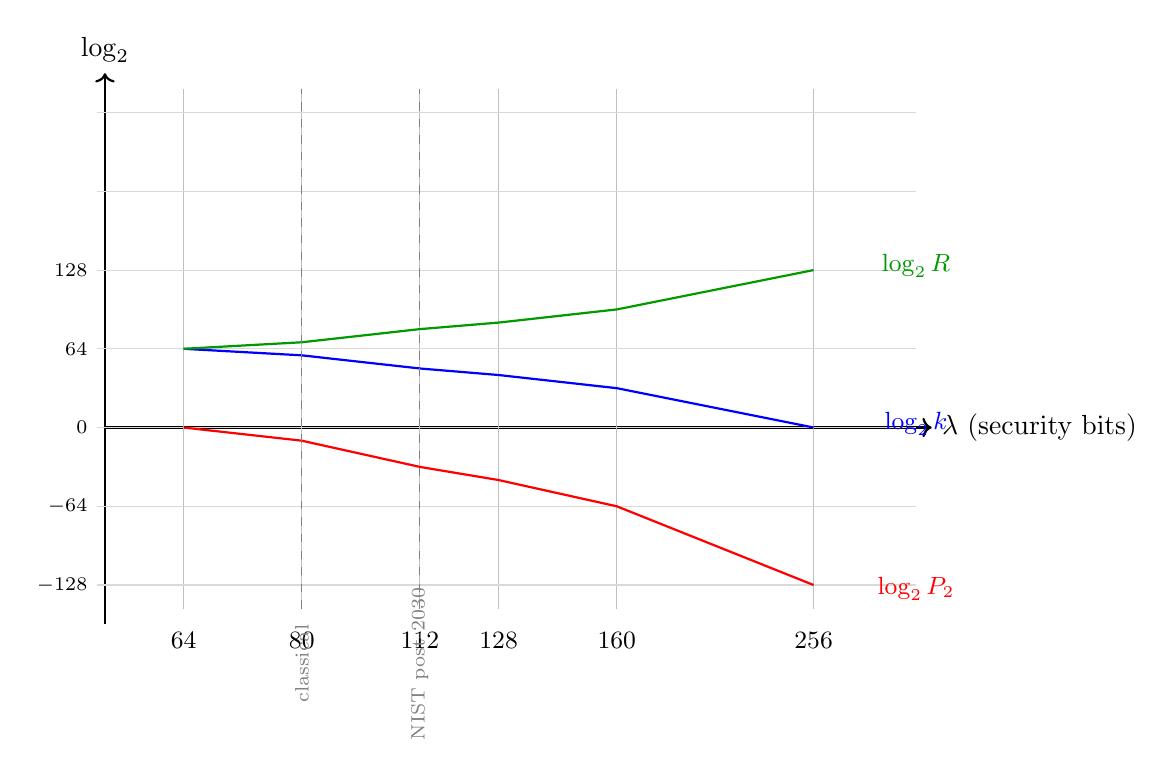
\begin{tikzpicture}[scale=1.0]
  % Axes
  \draw[->, thick] (0, 0) -- (10.5, 0) node[right] {$\lambda$ (security bits)};
  \draw[->, thick] (0, -2.5) -- (0, 4.5) node[above] {$\log_2$};

  % Lambda gridlines
  \foreach \x/\lab in {1/64, 2.5/80, 4/112, 5/128, 6.5/160, 9/256} {
    \draw[gray!50] (\x, -2.3) -- (\x, 4.3);
    \node[font=\small] at (\x, -2.7) {\lab};
  }

  % Y gridlines
  \foreach \y/\lab in {-2/-128, -1/-64, 0/0, 1/64, 2/85, 3/96, 4/128} {
    \draw[gray!30] (-0.1, \y) -- (10.3, \y);
  }

  % log_2 k
  \draw[blue, thick] (1, 1) -- (2.5, 0.917) -- (4, 0.75) -- (5, 0.667) -- (6.5, 0.5) -- (9, 0);
  \node[blue, font=\small] at (10.3, 0.05) {$\log_2 k$};

  % log_2 P_2
  \draw[red, thick] (1, 0) -- (2.5, -0.167) -- (4, -0.5) -- (5, -0.667) -- (6.5, -1) -- (9, -2);
  \node[red, font=\small] at (10.3, -2.05) {$\log_2 P_2$};

  % log_2 R
  \draw[green!60!black, thick] (1, 1) -- (2.5, 1.083) -- (4, 1.25) -- (5, 1.333) -- (6.5, 1.5) -- (9, 2);
  \node[green!60!black, font=\small] at (10.3, 2.05) {$\log_2 R$};

  % Annotations
  \draw[dashed, gray] (4, -2.3) -- (4, 4.3);
  \node[font=\scriptsize, gray, rotate=90] at (4, -3.0) {NIST post-2030};

  \draw[dashed, gray] (2.5, -2.3) -- (2.5, 4.3);
  \node[font=\scriptsize, gray, rotate=90] at (2.5, -3.0) {classical};

  % Y labels
  \node[font=\scriptsize, anchor=east] at (-0.1, -2) {$-128$};
  \node[font=\scriptsize, anchor=east] at (-0.1, -1) {$-64$};
  \node[font=\scriptsize, anchor=east] at (-0.1, 0) {$0$};
  \node[font=\scriptsize, anchor=east] at (-0.1, 1) {$64$};
  \node[font=\scriptsize, anchor=east] at (-0.1, 2) {$128$};

\end{tikzpicture}
\caption{The compromise triangle: how the three key quantities ($\log_2 k$, $\log_2 P_2$, $\log_2 R$) shift with rising security level $\lambda$. Blue ($k$) decreases slowly, red ($P_2$) decreases fastest, green ($R$) grows slowly. Higher security $\Rightarrow$ smaller pool, smaller legitimate collision, larger asymmetry. No two of them can be "improved" simultaneously.}
\label{fig:lambda-tradeoff}
\end{figure}

\subsection{Why all of this is \emph{static}}

It is important to understand what the above says \emph{and what it does not}. It says: if Alice, Bob, and Eve each independently and once pick their $k$-element sets, the odds ratio is $R \approx n/k$. That is a \emph{single event}.

What it does not say: how things work when a protocol runs \emph{across many rounds}, when the parties' internal states evolve, when they exchange signals, when the adversary accumulates observations. That is the \emph{dynamic} regime, and static analysis is not enough for it.

For a practical cryptographic protocol this is a problem: if we picked $\lambda = 80$ and so $k = 2^{58{,}67}$, $P_2 \approx 2^{-10{,}67}$, this means that on a single selection event Alice and Bob would collide with probability about $1/1\,627$. That is awful --- the protocol would fail in $99{,}94\%$ of cases. If we made $k$ large enough so that collision is certain ($k^2 \approx n$, i.e.\ $k \approx 2^{64}$), the adversary's chance jumps to $k^3/n^2 = 2^{-128} \cdot k = 2^{-64}$ --- a poor tradeoff.

\begin{aha}[Static alone is not enough]
The static bound gives us a \emph{ceiling} on the adversary's knowledge, not a practical protocol. A practical protocol has to find a way to \emph{reliably} (close to $100\%$) discover the intersection element without degrading $R$. In other words: it has to transform a static one-shot event into a dynamic, repeated process that \emph{preserves and amplifies} the asymmetry.
\end{aha}

That is exactly what the four design decisions in Chapter~\ref{pop:transformation} do.

\medskip
\noindent\textit{The static asymmetry tells us what the structural advantage is. The dynamic system shows us how to grasp it.}

\section{Four design decisions}\label{pop:transformation}

In Section~\ref{pop:static} we ran into a practical problem: the static asymmetry $R \approx n/k$ exists, but for a practical protocol it is worthless --- with a reasonable $\lambda$ Alice and Bob would in $99{,}94\%$ of cases fail to share even a single intersection element. We therefore need something that \emph{preserves} the static asymmetry (the adversary stays at a disadvantage) and at the same time \emph{amplifies} it (the legitimate parties achieve near-certain agreement).

That is the transformation problem of Grata Cascade. It splits into three sub-problems:

\begin{enumerate}[leftmargin=*]
\item \textbf{Communication without revealing.} The parties have to publicly exchange enough information to discover what they share, but not so much that Eve can discover it too.
\item \textbf{The adversary stays at the static bound.} No additional round of communication may move Eve into a better position than the one given by the ratio $R$. No accumulation effects, no leaks across time.
\item \textbf{The key requires knowledge of the intersection.} The final cryptographic key must be derivable \emph{only} from the intersection elements themselves --- not from what is visible on the wire.
\end{enumerate}

Grata Cascade addresses these three sub-problems with \emph{four} design decisions. Each one is, on its own, simple; combining them \emph{together} into a working CKA protocol is non-trivial. Let us walk them one at a time.

\subsection{Decision 1: Hash as a one-way commitment}\label{pop:design-hash}

\paragraph{Problem.} Alice holds a private pool $\mathcal{V}_A$ in memory (say, thousands of 32-byte vectors). Bob holds his own $\mathcal{V}_B$. They want to exchange information about what they have \emph{in common} without that shared material ever appearing on the public wire. How?

\paragraph{Solution.} Alice computes the SHA-256 hashes of all her vectors and sends \emph{prefixes} of those hashes (e.g.\ the first 5 bytes --- not the full hash). Bob hashes his own vectors and looks for any whose prefix matches what he received. If he finds one, it is a candidate for a shared vector.

\begin{aha}[A hash is a one-way commitment]
SHA-256 is \emph{one-way}: from input you can compute the hash easily, but the inverse is not feasible. When Alice sends $h(v) = $ "f3a2..." it reveals \emph{almost nothing} about $v$, except that it exists. But when Bob holds his own $v'$ and computes $h(v') = $ "f3a2...", he immediately knows that $v = v'$. Nothing was disclosed publicly; in private they have agreed.
\end{aha}

\paragraph{Nuance: truncated hashes.} Alice does not send the full 32-byte hash, only the first few bytes. Why?

\begin{itemize}[leftmargin=*]
\item \textbf{Full hash} (32 bytes): Bob almost never finds an accidental match, but Alice has to transmit $32 \cdot |\mathcal{V}_A|$ bytes per round --- expensive in bandwidth.
\item \textbf{Short hash} (e.g.\ $h_{AB} = 5$ bytes): Bob finds more \emph{candidate} matches (some are spurious, false positives), but bandwidth is cut to $5/32$. The spurious matches are then \emph{cascaded out} in the remaining decisions (3 and 4).
\end{itemize}

In reference configuration v2 we use three different lengths for three roles:
\begin{itemize}[leftmargin=*]
\item $h_{AB} = 5$ bytes: prefix Alice sends to Bob (step A$\to$B).
\item $h_{BA} = 2$ bytes: prefix Bob sends back to Alice (step B$\to$A) saying "I found these candidates".
\item $h_P = 8$ bytes: prefix for \emph{password} vectors (cross-round vectors with longer-term significance).
\end{itemize}

Adding these up gives the \textbf{cumulative preimage barrier} $\lambda = 8 \cdot (5 + 2 + 8) = 120$ bits. That is how many bits the adversary has to "guess on top of" a single vector to make it through the entire cascade. A huge fence.

\begin{sidebar}[Historical context: Merkle puzzles]
The principle of "key agreement via a public hash function" goes back to Merkle puzzles (1978): Alice sends $N$ puzzles at $O(N)$ work each, Bob solves one in $O(N)$, Eve has to inspect them all in $O(N^2)$. Impagliazzo and Rudich (1989) showed $O(N^2)$ is optimal in the black-box model. Grata Cascade extends this lineage: combined with the other decisions it conjecturally pushes the adversary's work \emph{above} $O(N^2)$. Full discussion in the main paper.
\end{sidebar}

\subsection{Decision 2: Public drift via a random vector}\label{pop:design-drift}

\paragraph{Problem.} Alice and Bob have their private pools. After the first round they already know something about each other. In the next round they \emph{have to} update their pools somehow --- otherwise they would just repeat themselves and the entire game would be the same. But how to update them so that:
\begin{itemize}[leftmargin=*]
\item Alice's and Bob's pools stay \emph{correlated} (otherwise they have nothing to agree on)?
\item Eve cannot \emph{see} which vectors each of them holds?
\end{itemize}

\paragraph{Solution.} In each round a \emph{public random vector} $R_t$ is generated (by some standard cryptographically random procedure). Alice sees it, Bob sees it, Eve also sees it. Alice and Bob each apply an identical update rule that uses $R_t$ to \emph{shift} their pools. Although Eve sees $R_t$, she does \emph{not see} which specific vectors Alice or Bob held, so she cannot reconstruct the pools.

\begin{aha}[We all see the same map; each of us walks a different path]
$R_t$ is public. The update rule is public. The Stat distribution that emerges is public --- Eve can compute it exactly. What is \emph{not} public: the specific paths Alice and Bob walked through that distribution. They have an identical map but each sees it "from their own position".
\end{aha}

That is a subtle but key point. Eve can build a perfect picture of the \emph{statistical space}, but not of the \emph{specific points} in it that belong to the parties. So she can attack only probabilistically --- and the probability of hitting a specific vector stays at $1/n$, because the vector itself evolves under $R_t$, which is uniformly random.

\paragraph{Probabilistic update.} A second protective layer: the update of each vector happens with probability $p_\text{upd} < 1$. In reference v2, $p_\text{upd} = 0{,}75$. This means some vectors are \emph{not updated} in a given round. Eve knows that $75\%$ of vectors were updated, but does not \emph{which ones}. A statistical mask hiding the specific state from the adversary.

\subsection{Decision 3: The update rule (TPM-inspired)}\label{pop:design-update}

\paragraph{Problem.} Given a public $R_t$, and given that we want each side to update its own vectors, what concrete rule should we pick? It has to satisfy two conditions: (a) it has to gradually align Alice's and Bob's pools (otherwise they will never agree), (b) it must not leak the gradient (which direction a vector moved).

\paragraph{Inspiration.} Grata Cascade draws on a historical protocol called the \textbf{Tree Parity Machine} (TPM, 2002), in which two neural networks gradually synchronised their weights. TPM was later broken by a \emph{geometric attack} (Klimov-Mityagin-Shamir 2003): from the synchronisation messages the adversary could reconstruct the weights because of gradient leakage.

Grata Cascade borrows the structure (iterative synchronisation through a shared signal) but \emph{does not leak the gradient}. The rule is deterministic and simple:

\[
v_i \gets \begin{cases} v_i + R_i - 128 & \text{if the result is in the range } [0, 255], \\ R_i & \text{otherwise (overflow branch)}. \end{cases}
\]

(Each vector component is a byte $\in [0, 255]$. Shifting by $R_i - 128$ centres the update around zero: sometimes up, sometimes down.)

\begin{aha}[Same music, different choreography]
Alice and Bob hear the same song ($R_t$). They apply the same dance rule. But their starting positions (private vectors) differ, so they end up in different places. Eve hears the song but does not know where Alice and Bob started --- so she cannot tell where they end.
\end{aha}

That is the structural difference from TPM: there, synchronisation between the networks revealed the gradient (which direction the weights moved). Here, no shared information \emph{between Alice and Bob} is involved. They both just apply the same public update.

\subsection{Decision 4: AES without padding (no validation oracle)}\label{pop:design-aes}

\paragraph{Problem.} After several rounds Alice and Bob hold a list of candidate "password vectors" --- vectors that have passed all the filters and are likely part of their intersection. From those vectors they both have to derive the same \emph{final key} $K^*$.

A naive solution: Alice computes $K^* = \text{SHA-256}(v_1 \Vert v_2 \Vert \cdots \Vert v_M)$ and Bob does the same. If they have the same vectors, they get the same key. Works.

But what if Eve has a pool of $10^{15}$ candidate vectors? She could try millions of combinations, compute the hashes, and possibly find $K^*$. How do we deter her?

\paragraph{Solution.} Instead of sending vectors directly, Alice encrypts them using AES in CBC mode \emph{without padding} (\texttt{PaddingMode.None}). This has two key properties:

\begin{enumerate}[leftmargin=*]
\item \textbf{No validation oracle.} With normal padding (PKCS7), a wrong key is detectable: decryption produces invalid padding, ending the guessing game. \emph{Without padding} a wrong-key decryption produces pseudo-random bytes, indistinguishable from a correct decryption. Eve has no way to verify whether her key guess is correct.
\item \textbf{Indistinguishable candidate set.} For a 32-byte vector, the probability that a random candidate "looks plausible" is $2^{-\lambda} = 2^{-120}$. But the total space of possible vectors is $2^{8 \cdot 32} = 2^{256}$. After the preimage barrier there remain $2^{256-120} = 2^{136}$ candidates, all of whom \emph{look equally plausible}. Eve cannot prefer any one of them.
\end{enumerate}

\begin{aha}[A heap of identical keys, many dead-end corridors]
Imagine a bunch of $2^{136}$ identical-looking keys. They all open the \emph{same door}, but past the door the paths split --- each key leads into its own corridor ($2^{136}$ corridors in total). All but one are dead ends; only one leads to the secret. Eve unlocks the door with her key and finds herself in some corridor --- bare walls, no signs, no way to tell whether it is a dead end. All the corridors look identical. AES without padding produces exactly this situation: every key guess decrypts something, but the output is 32 bytes of pseudo-random noise, indistinguishable from the noise produced by other guesses.
\end{aha}

\subsection{The combined system: how they fit together}\label{pop:design-combined}

These four decisions \emph{cascade} to take us from the static into the dynamic regime. Each decision addresses one specific attack vector:

\begin{itemize}[leftmargin=*]
\item \textbf{Hash addressing} blocks the direct compute attack: even with unlimited time, SHA-256 cannot be inverted.
\item \textbf{Public drift} blocks accumulation attacks: Eve sees all the $R_t$, but the parties' specific pools stay invisible.
\item \textbf{The update rule} blocks gradient leakage (the TPM lesson): synchronisation gives Eve no information about trajectories.
\item \textbf{AES without padding} blocks flooding by candidates: even with a million vectors, Eve has no validation oracle.
\end{itemize}

\begin{table}[ht]
\centering
\small
\begin{tabular}{lll}
\toprule
Aspect & Static (Birthday) & Dynamic (Grata Cascade) \\
\midrule
Selection & Random, one-shot & Iterative, drift-driven \\
Universe & Fixed, $|U| = n$ & Effectively narrowed via Stat \\
Party correlation & None & Synchronised via $R_t$ \\
Goal & Set intersection & A specific sequence of hash hits \\
Adversary's position & Third party in the same game & Observer without coherent state \\
\bottomrule
\end{tabular}
\caption{The static birthday model versus the dynamic Grata Cascade system. The dynamic mechanisms \emph{strengthen} the static foundation but do not break it --- the adversary stays at the asymmetry ratio $R \approx n/k$ as a lower bound on the legitimate parties' advantage.}
\label{tab:pop-static-vs-dynamic}
\end{table}

\begin{figure}[h]
\centering
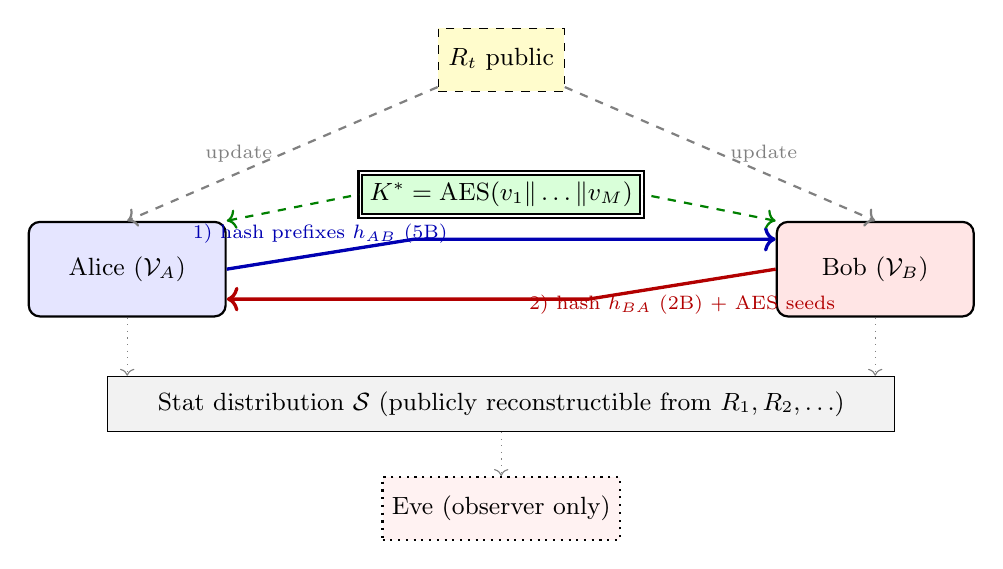
\begin{tikzpicture}[scale=0.95, font=\small]
  % Parties
  \node[draw, rounded corners, thick, fill=blue!10, minimum width=2.5cm, minimum height=1.2cm] (alice) at (0, 0) {Alice ($\mathcal{V}_A$)};
  \node[draw, rounded corners, thick, fill=red!10, minimum width=2.5cm, minimum height=1.2cm] (bob) at (10, 0) {Bob ($\mathcal{V}_B$)};

  % R_t public input
  \node[draw, dashed, fill=yellow!20, minimum width=1.6cm, minimum height=0.8cm] (rt) at (5, 2.8) {$R_t$ public};

  % Update arrows from R_t
  \draw[->, dashed, thick, gray] (rt) -- node[left, font=\scriptsize] {update} (alice.north);
  \draw[->, dashed, thick, gray] (rt) -- node[right, font=\scriptsize] {update} (bob.north);

  % A->B communication (hash AB)
  \draw[->, very thick, blue!70!black] (alice.east) -- ++(2.5, 0.4)
    node[midway, above, font=\scriptsize] {1) hash prefixes $h_{AB}$ (5B)} -- ($(bob.west)+(0,0.4)$);

  % B->A communication (hash BA + AES seeds)
  \draw[->, very thick, red!70!black] (bob.west) -- ++(-2.5, -0.4)
    node[midway, below, font=\scriptsize] {2) hash $h_{BA}$ (2B) + AES seeds} -- ($(alice.east)+(0,-0.4)$);

  % Stat distribution below
  \node[draw, fill=gray!10, minimum width=10cm, minimum height=0.7cm] (stat) at (5, -1.8) {Stat distribution $\mathcal{S}$ (publicly reconstructible from $R_1, R_2, \ldots$)};

  % Arrows into stat
  \draw[->, dotted, gray] (alice.south) -- (stat.north -| alice.south);
  \draw[->, dotted, gray] (bob.south) -- (stat.north -| bob.south);

  % Eve
  \node[draw, dotted, thick, fill=red!5, minimum width=2cm, minimum height=0.8cm] (eve) at (5, -3.2) {Eve (observer only)};
  \draw[->, dotted, gray] (stat.south) -- (eve.north);

  % Output key
  \node[draw, double, thick, fill=green!15, minimum width=2cm] (key) at (5, 1.0) {$K^* = \text{AES}(v_1 \Vert \ldots \Vert v_M)$};
  \draw[<-, thick, green!50!black, dashed] (alice.north east) -- (key.west);
  \draw[<-, thick, green!50!black, dashed] (bob.north west) -- (key.east);

\end{tikzpicture}
\caption{The combined dynamic system in one round. The public $R_t$ updates both pools identically. Alice sends Bob hash prefixes $h_{AB}$ (decision 1, step 1). Bob returns hashes $h_{BA}$ and AES-encrypted seeds (decisions 1+4, step 2). The Stat distribution is reconstructible by Eve, but the specific pools are not (decision 2). After several rounds Alice and Bob both finalise $K^*$ from the available password vectors (decision 4).}
\label{fig:combined-system}
\end{figure}

In Chapter~\ref{pop:protocol} we look at the concrete implementation in more detail: what Alice does in step 1, what Bob sends in step 2, what the Stat table looks like, and how the final key is derived. Chapters~\ref{pop:drift} and~\ref{pop:aes} put decisions 2+3 (drift) and 4 (AES) under a more detailed microscope.

\medskip
\noindent\textit{Statics gives the bound. Drift gives the dynamics. The hash gives one-wayness. AES without padding gives indistinguishability. Together: convergence and security.}

\section{The protocol in action}\label{pop:protocol}

In Chapter~\ref{pop:transformation} we walked through \emph{what} the four design decisions do. This chapter shows \emph{how} they apply in one round of the protocol: who sends what to whom, in what order, with what parameters. Goal: after reading this, you should be able to look at the code or paper v9 §5 and know what each parameter is responsible for.

\subsection{Thirteen parameters (and what they do)}

Table~\ref{tab:pop-params} lists all 13 parameters of reference v2. Bold values are those that were empirically calibrated (not just "reasonably chosen"). Each row gets a brief plain-language note about what happens if you raise or lower it.

\begin{table}[ht]
\centering
\small
\begin{tabular}{lll}
\toprule
Symbol & Value & What it does (and what happens if you change it) \\
\midrule
$L$ & 32 B & Vector length (32 bytes). Larger $\Rightarrow$ exponentially more indistinguishability, but more memory. \\
$N$ & 4096 & Vectors per side. Larger $\Rightarrow$ more match candidates, but more bandwidth per round. \\
$h_{AB}$ & 5 B & A$\to$B hash prefix. Short $\Rightarrow$ false collisions and silent failures. Long $\Rightarrow$ too much bandwidth. \\
$h_{BA}$ & 2 B & B$\to$A hash prefix. \emph{Deliberately short} for the flooding defense (see §\ref{pop:aes}). \\
$h_P$ & \textbf{8 B} & Password hash. Cross-round identifier. Long for production reliability. \\
$M$ & \textbf{8} & Password candidates per round. More $\Rightarrow$ combinatorics blow up for the adversary. \\
$s$ & \textbf{4} & Seed perturbation ($\pm s$). Validated empirically neutral in $[1, 30]$. \\
$p_\text{upd}$ & \textbf{0{,}75} & Per-vector update probability per round. Range $[0{,}6, 0{,}95]$ enforced. \\
$\tau$ & $-512$ & Termination threshold ($\log_2$). When the accumulated password log-probability drops below this, we stop. \\
$\theta_\text{cut}$ & $-8$ & Pool threshold. Structurally inactive in ref v2 ($\log_2 \Pr$ of vectors $\approx -256$). \\
$\theta_\text{cand}$ & \textbf{$-8$} (off) & Tier-3 candidate filter. Default equal to $\theta_\text{cut}$, i.e.\ disabled. \\
$\text{MaxIter}$ & \textbf{500} & Iteration cap. Median convergence on reference v2 is $\approx 49$ iterations. \\
\bottomrule
\end{tabular}
\caption{The 13 parameters of Grata Cascade reference v2 (after the 2026-05-02 pivot). Bold values are empirically calibrated by systematic sweeps. The range $p_\text{upd} \in [0{,}6, 0{,}95]$ is enforced at config load time: below 0{,}6 the protocol does not converge; above 0{,}95 Stat collapses and the adversary's direct sampling becomes effective.}
\label{tab:pop-params}
\end{table}

Combined, $h_{AB} + h_{BA} + h_P = 5 + 2 + 8 = 15$ bytes $\Rightarrow$ \textbf{cumulative preimage barrier} $\lambda = 120$ bits (recall Chapter~\ref{pop:transformation}). That is how many bits the adversary has to overcome per password vector.

\subsection{Five parametric profiles}

One protocol, several situations --- so Grata Cascade is a \emph{family} of configurations, not a single fixed implementation. Currently the repo carries:

\begin{itemize}[leftmargin=*]
\item \textbf{\texttt{reference}} (v2): production baseline, fully empirically validated.
\item \textbf{\texttt{low\_resource\_iot}}: for IoT devices, $L = 16$, $N = 1024$ --- less memory, weaker preimage ($\lambda = 96$ bits).
\item \textbf{\texttt{high\_security\_pq128}}: paranoid post-quantum variant, $L = 64$, $N = 8192$, $h_{AB} = 6$ --- 128-bit security but $\sim 64$ s per round (vs.\ $\sim 1$ s for reference).
\item \textbf{\texttt{break\_demo}} (research): \emph{deliberately weakened} version for pedagogical attack demos, $L = 8$, $h_{AB} = 3$, $\lambda = 56$ bits. Not for production.
\item \textbf{\texttt{reference\_h\_AB6}} (v3 candidate): a clone of reference with $h_{AB} = 5 \to 6$ ($\lambda = 128$ bits). Validated by a 50k-run ablation (see §\ref{pop:empirical}).
\end{itemize}

The profile \texttt{reference\_h\_AB6} is the newest and most promising: it strengthens $\lambda$ to 128 bits at the cost of $+4$ KB/round bandwidth, achieving 0 divergences over 50k runs. If the user accepts the bandwidth tradeoff, it is a natural candidate for the "v3 reference".

\subsection{What exactly happens in one round}\label{pop:round-walkthrough}

Let us walk through the steps of one round $t$. We assume initialised pools $\mathcal{V}_A$, $\mathcal{V}_B$ (each 4096 random 32-byte vectors) and an initialised Stat table $\mathcal{S}$ (uniform).

\paragraph{Step 1: A sends hashes.}
Alice computes the SHA-256 hash of each vector in her pool and truncates to the first 5 bytes ($h_{AB}$). The resulting list $\{H[0\mathord{:}5](v) : v \in \mathcal{V}_A\}$ contains 4096 hash prefixes, 5 B each. That is $4096 \cdot 5 = 20$ KB --- the largest message of the entire round. It goes to Bob.

\paragraph{Step 2: B looks for collisions.}
Bob walks through his pool, hashes his own vectors, and looks for prefixes that match those received from Alice. This produces some number of \emph{candidate collisions}. Of these:
\begin{enumerate}[leftmargin=*]
\item He sorts them ascending by their probability under Stat $\mathcal{S}_B$ (lowest probability first --- this is tail selection, see §\ref{pop:drift}).
\item He optionally filters by the threshold $\theta_\text{cand}$ (off in the reference).
\item He picks the first $M = 8$ candidates.
\end{enumerate}
These candidates are \emph{likely} to be in the intersection with Alice's pool (their hashes match) and \emph{likely} to be statistically atypical (tail).

\paragraph{Step 3: B sends back.}
Bob sends Alice three things:
\begin{itemize}[leftmargin=*]
\item The public random vector $R_t$ (32 B) --- input to the Stat update.
\item B$\to$A hash prefixes of these candidates: $\{H[5\mathord{:}7](v) : v \in \text{candidates}\}$ ($M \cdot h_{BA} = 16$ B).
\item AES-encrypted seed $\sigma_t$, under the key $K_t = H(v_{\pi(1)} \Vert \cdots \Vert v_{\pi(M)})$ (32 B).
\end{itemize}

\paragraph{Step 4: A decrypts and updates.}
Alice enumerates which combinations of 8 vectors from her pool match the received B$\to$A hashes. For each candidate combination she computes a candidate $K_t'$, attempts AES decryption (\emph{always succeeds syntactically}, due to NoPadding), and obtains a candidate seed $\sigma_t'$. Without padding she has no way to verify which is correct --- she carries multiple candidates forward.

Then: both sides apply a \emph{deterministic} Stat update from $R_t$ and update their pools with probability $p_\text{upd} = 0{,}75$ (perturbation $\pm s = \pm 4$, filtered by $\theta_\text{cut}$).

\paragraph{Step 5: Termination.}
B maintains an accumulating list $\mathcal{P}$ of password vectors (those that have appeared in the candidate set). When the sum of $\log_2 \Pr_{\mathcal{S}_B}(v)$ over $v \in \mathcal{P}$ drops below $\tau = -512$, we stop. B sends the Final message containing $h_P = 8$-byte hashes of all $|\mathcal{P}|$ password vectors.

A enumerates combinations of her candidate seeds, looking for those whose $h_P$ hashes match. The final key:
\[
K^* = H(v_{\pi(1)} \Vert v_{\pi(2)} \Vert \cdots \Vert v_{\pi(|\mathcal{P}|)}).
\]

A median session takes $\approx 49$ rounds. Bandwidth per round is $\approx 20{,}5$ KB. Whole session: about $1$ MB.

\subsection{Visualisation: one round at a glance}

\begin{figure}[h]
\centering
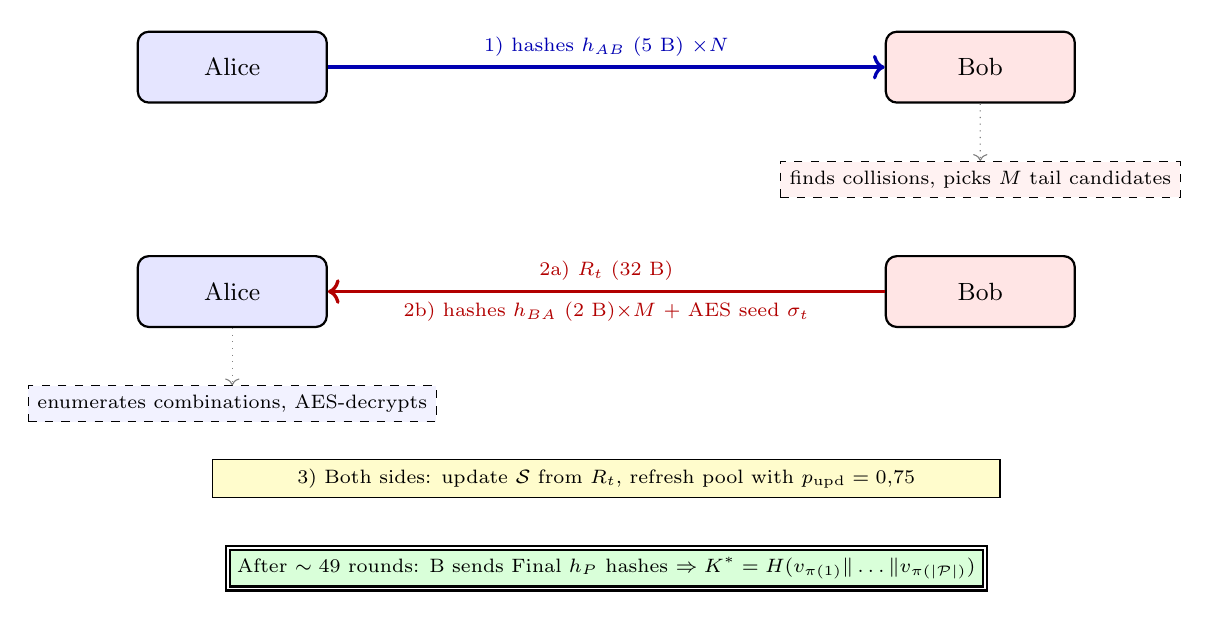
\begin{tikzpicture}[scale=0.95, font=\small,
    party/.style={draw, rounded corners, thick, minimum width=2.4cm, minimum height=0.9cm},
    msg/.style={->, very thick}]

  % Parties
  \node[party, fill=blue!10] (a1) at (0, 5) {Alice};
  \node[party, fill=red!10] (b1) at (10, 5) {Bob};

  % Step 1: A sends hashes
  \draw[msg, blue!70!black] (a1.east) -- node[above, font=\scriptsize] {1) hashes $h_{AB}$ (5 B) $\times N$} ($(b1.west)+(0,0)$);

  % B selects candidates
  \node[draw, dashed, fill=red!5, minimum width=4cm, font=\scriptsize] (bcand) at (10, 3.5) {finds collisions, picks $M$ tail candidates};
  \draw[->, dotted, gray] (b1) -- (bcand);

  % Step 2: B sends back
  \node[party, fill=blue!10] (a2) at (0, 2.0) {Alice};
  \node[party, fill=red!10] (b2) at (10, 2.0) {Bob};
  \draw[msg, red!70!black] (b2.west) --
    node[above, font=\scriptsize] {2a) $R_t$ (32 B)}
    node[below, font=\scriptsize] {2b) hashes $h_{BA}$ (2 B)$\times M$ + AES seed $\sigma_t$}
    (a2.east);

  % A decrypts
  \node[draw, dashed, fill=blue!5, minimum width=4cm, font=\scriptsize] (adec) at (0, 0.5) {enumerates combinations, AES-decrypts};
  \draw[->, dotted, gray] (a2) -- (adec);

  % Update Stat
  \node[draw, fill=yellow!20, minimum width=10cm, font=\scriptsize] (stat) at (5, -0.5) {3) Both sides: update $\mathcal{S}$ from $R_t$, refresh pool with $p_\text{upd} = 0{,}75$};

  % After N rounds
  \node[draw, double, thick, fill=green!15, font=\scriptsize, minimum width=6cm] (key) at (5, -1.7) {After $\sim 49$ rounds: B sends Final $h_P$ hashes $\Rightarrow K^* = H(v_{\pi(1)} \Vert \ldots \Vert v_{\pi(|\mathcal{P}|)})$};

\end{tikzpicture}
\caption{Anatomy of one round. Step 1: Alice sends 4096 truncated hashes (20 KB). Step 2: Bob finds collisions, picks $M=8$ tail candidates, sends back $R_t$ + $h_{BA}$ hashes + AES seed. Step 3: both sides update Stat. After $\sim 49$ rounds: termination.}
\label{fig:round-anatomy}
\end{figure}

\subsection{Three roles for hashes, three different calibration constraints}\label{pop:hash-rationale}

The three hash lengths $h_{AB}$, $h_{BA}$, $h_P$ are \emph{not} just calibration knobs sharing a single "security" semantics. Each plays a different role and is calibrated against a different constraint:

\begin{itemize}[leftmargin=*]
\item \textbf{$h_{AB}$ as a correctness floor.} Too short an $h_{AB}$ makes random B-vectors accidentally match A-hashes (false collisions), and Bob ends up building a seed on top of wrong vectors. That is a \emph{silent failure} with no recovery path. The calibration formula is $h_{AB} \geq \lceil (2 \log_2 N + 8)/8 \rceil$. For $N = 4096$ this gives $h_{AB} \geq 4$; the reference uses 5 (with an 8-bit margin).

\item \textbf{$h_{BA}$ as a deliberately permissive filter.} \emph{Shorter is better.} A longer $h_{BA}$ would leave the adversary with a unique candidate when running a large pool, which she could then verify in subsequent rounds. A short $h_{BA}$ \emph{deliberately} keeps the number of stage-b survivors above 1 even for extreme pools $\Rightarrow$ flooding rather than identification. Detail in §\ref{pop:aes}.

\item \textbf{$h_P$ as cross-round synchronisation.} After $\sim 50$ rounds Alice has accumulated a candidate pool of $\sim 400$ vectors. $h_P$ has to be long enough so that Final hashes uniquely identify the password vectors without silent key-mismatches. For $h_P = 8$ B and a 50-round session: expected silent mismatch $\approx 1{,}7 \cdot 10^{-16}$ per session.
\end{itemize}

These three different constraints explain why ref v2 does not have $h_{AB} = h_{BA} = h_P = 8$ B (as a naive user might want) --- that would yield $\lambda = 192$ bits, but $h_{BA} = 8$ B would weaken the flooding defense to "specific identification" and break the design. Per-role calibration is structural, not cosmetic.

\subsection{Adversary model}

For completeness: who is the assumed adversary.

Grata Cascade is designed for \emph{passive adversaries}: they see all public messages (the transcript, $R_t$ vectors, AES ciphertexts, Final hashes), they have PPT (probabilistic polynomial time) compute resources. The adversary may even be a quantum computer.

\textbf{Out of scope:} an active network adversary who could modify messages in transit. Grata Cascade is meant to run \emph{inside} an authenticated transport (TLS, Noise framework). There the transport layer takes care of message integrity and peer authentication. An active adversary capable of bypassing transport authentication has strictly greater access than any specific Grata-Cascade-level attack would add.

In Chapter~\ref{pop:empirical} we will see \emph{five concrete classes} of passive adversaries (B.1, B.2, B.3, B.4, B.7) against which the protocol stood up.

\section{Statistical drift}\label{pop:drift}

In Chapter~\ref{pop:transformation} we said that "public drift via a random vector" is decision 2. Here we look at it more closely: what the shared statistical distribution $\mathcal{S}$ looks like, why the legitimate parties pick "tail" candidates, and why there is a narrow operating range for $p_\text{upd}$.

\subsection{Stat: a publicly reconstructible map}\label{pop:stat-map}

Each side (Alice and Bob) keeps a local table $\mathcal{S}$. For each of the $L = 32$ vector positions it holds a single probability distribution over 256 possible byte values. Concretely: $p_i(x)$ tells you how likely position $i$ is to hold byte value $x$. Initially every distribution is uniform --- $p_i(x) = 1/256$ for all $x$ (no value is special).

As rounds progress the distributions \emph{concentrate}: some byte values gain probability, others lose it. That is the "drift" in this chapter's title. Let us look at how it works.

\paragraph{The update rule.} When a new $R_t$ arrives, both sides perform three steps for each position $i$:

\begin{enumerate}[leftmargin=*]
\item Take the old distribution $p_i$ (256 numbers summing to 1).
\item Build the \emph{shifted} distribution $\tilde{p}_i$. The shift mirrors the vector update rule from §\ref{pop:design-update}: if a vector held value $v$ at position $i$, after the update it holds $v + R_{t,i} - 128$ (when the result lies in $[0, 255]$) or $R_{t,i}$ (overflow branch). $\tilde{p}_i(x)$ is the probability that, after this operation, the byte ends up at value $x$.
\item Mix in the ratio $p_\text{upd} : (1 - p_\text{upd})$:
\[
p_i'(x) = p_\text{upd} \cdot p_i(x) + (1 - p_\text{upd}) \cdot \tilde{p}_i(x).
\]
For reference v2, $p_\text{upd} = 0{,}75$, so the \emph{old} distribution gets weight 75 \% and the \emph{shifted} one weight 25 \%.
\end{enumerate}

The probability of a whole vector $v$ is then the product across positions: $\Pr_\mathcal{S}(v) = \prod_i p_i(v_i)$.

\begin{sidebar}[Concrete shift example]
Suppose $R_{t,i} = 200$ at position $i$. The shift is $200 - 128 = +72$. Then:
\begin{itemize}[leftmargin=*]
\item Mass that sat on values $0$--$183$ moves to values $72$--$255$ (a $+72$ shift).
\item Mass on values $184$--$255$ would flow outside the byte range ($256$--$327$). Instead the overflow branch collects all of it and dumps it onto value $200$ (= $R_{t,i}$).
\item The resulting shifted distribution $\tilde{p}_i$ has a translated piece and a "spike" at one point. We then mix it $0{,}75 : 0{,}25$ with the old distribution.
\end{itemize}
The drift across many rounds is the accumulation of these shifts and overflow spikes. We start uniform, but every $R_t$ pours a small drop of mass onto a specific value, and after dozens of rounds these drops compose into the structure shown in Figure~\ref{fig:stat-evolution}.
\end{sidebar}

\begin{aha}[Stat being public is not the same as compromise]
$\mathcal{S}$ is a \emph{deterministic function} of the public sequence $R_1, R_2, \ldots$ The adversary can compute it \emph{exactly} like Alice and Bob. This is not a problem. The problem would arise only if the adversary knew \emph{which vectors} Alice and Bob updated. But she does not, because each vector is updated with probability $p_\text{upd} < 1$ independently.
\end{aha}

That distinction between "distributional knowledge" (shared by all including the adversary) and "trajectory knowledge" (private to each party) is key. The adversary sees a coverage map but does not know where Alice and Bob actually stand on it.

\subsection{Inverse-probability selection}

When in step 2 (see §\ref{pop:round-walkthrough}) Bob picks $M = 8$ password candidates from his hash collisions, he sorts them ascending by probability under $\mathcal{S}_B$ and picks the \emph{lowest}. That means candidates with the \emph{smallest} probability under the current distribution --- the "tail".

\paragraph{Why tail and not the typical centre?} Picture a \emph{wheel of fortune} with 256 sectors --- one for each byte value. The sectors are not equal in size: a sector's area is proportional to $p_i(x)$ from the distribution $\mathcal{S}$. Some sectors are fat wedges (typical values with high $p$), others are slivers barely visible (tail values with low $p$). Anyone who knows the public sequence $R_t$ can build this wheel --- including the adversary.

\begin{itemize}[leftmargin=*]
\item \textbf{The adversary} spins the wheel: the ball lands in a sector proportionally to its size, so the overwhelming majority of the time it falls into some fat wedge. This is direct sampling from $\mathcal{S}$.
\item \textbf{Bob} does not spin: he \emph{deliberately points at the thinnest sliver}. The specific vector $v$ he picks has a probability $\approx 2^{-160}$ under $\mathcal{S}$ --- an utterly tiny sliver wedged between fat sectors.
\end{itemize}

That is the inverse-probability defense principle: Bob's strategy and the adversary's strategy are \emph{deliberately opposed}. From the same wheel each one aims for the opposite end.

\begin{aha}[Same wheel, opposite strategies]
The distribution $\mathcal{S}$ is a publicly reconstructible wheel that everyone sees the same way. But Bob points at the thinnest sliver, while the adversary's best direct sampling lands in a fat wedge. To hit Bob's pick without dumb luck, the adversary would have to \emph{enumerate} the slivers instead of spinning --- and there are exponentially many of them in a 32-byte space.
\end{aha}

For an inactive $\theta_\text{cand}$ filter (the reference v2 default) the typical numbers look like this: the median $\log_2 \Pr$ of Bob's candidates is $\approx -160$ bits, while the adversary's direct sampling from $\mathcal{S}$ on average lands at $\log_2 \Pr \approx -75$. Between $-75$ and $-160$ is a gulf of $2^{85}$ --- that is roughly the "distance" between the typical and tail regions in a 32-byte space.

\subsection{Operating range \texorpdfstring{$p_\text{upd} \in [0{,}6, 0{,}95]$}{p\_upd in [0.6, 0.95]}}

$p_\text{upd}$ is the probability that a given vector is updated in a given round. In reference v2, $p_\text{upd} = 0{,}75$. Empirical sweeps reveal a very narrow operating window:

\begin{itemize}[leftmargin=*]
\item \textbf{$p_\text{upd} \leq 0{,}5$:} the drift forms too slowly. After $\sim 100$ rounds $\mathcal{S}$ is still close to uniform, there is no real difference between tail and centre, tail-selection does not pick structurally separated candidates $\Rightarrow$ \textbf{the protocol does not converge.}
\item \textbf{$p_\text{upd} = 0{,}75$ (sweet spot):} median convergence $\approx 49$ rounds, $\mathcal{S}$ entropy $\approx 7{,}55$ bit/byte, tail candidates $\log_2 \Pr \approx -160$.
\item \textbf{$p_\text{upd} \geq 0{,}95$:} $\mathcal{S}$ collapses to a delta (per-byte max $p \to 1$), tail-selection loses its meaning, candidates concentrate in the "typical" region $\Rightarrow$ \textbf{direct sampling by the adversary becomes effective.}
\end{itemize}

\begin{warning}[The range is enforced at config load time]
Values outside $[0{,}6, 0{,}95]$ are actively rejected when loading the config (\texttt{configs/reference.json}). An attempt to instantiate with $p_\text{upd} = 1{,}0$ aborts the program with an explicit error. There is no \emph{silent} way to pick an unsafe value.
\end{warning}

\subsection{Visualisation: Stat distribution evolving across rounds}

\begin{figure}[h]
\centering
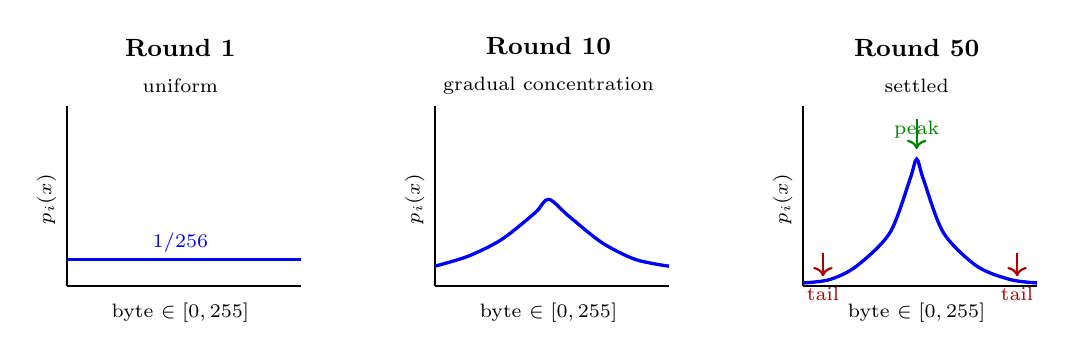
\begin{tikzpicture}[scale=0.85, font=\small]
  % Three panels: round 1, 10, 50; widened spacing, two-line titles
  \foreach \kolo/\offset in {0/0, 1/5.5, 2/11} {
    \begin{scope}[shift={(\offset, 0)}]
      % Two-line title: bold first line + scriptsize subtitle
      \ifnum\kolo=0
        \node[align=center] at (1.7, 3.3) {\bfseries Round 1\\[2pt]\normalfont\scriptsize uniform};
      \fi
      \ifnum\kolo=1
        \node[align=center] at (1.7, 3.3) {\bfseries Round 10\\[2pt]\normalfont\scriptsize gradual concentration};
      \fi
      \ifnum\kolo=2
        \node[align=center] at (1.7, 3.3) {\bfseries Round 50\\[2pt]\normalfont\scriptsize settled};
      \fi
      % Axes
      \draw[thick] (0, 0) -- (3.5, 0);
      \draw[thick] (0, 0) -- (0, 2.7);
      \node[font=\scriptsize] at (1.7, -0.4) {byte $\in [0, 255]$};
      \node[font=\scriptsize, rotate=90] at (-0.3, 1.3) {$p_i(x)$};

      % Distribution per round
      \ifnum\kolo=0
        \draw[blue, very thick] (0, 0.4) -- (3.5, 0.4);
        \node[blue, font=\scriptsize] at (1.7, 0.65) {$1/256$};
      \fi
      \ifnum\kolo=1
        \draw[blue, very thick, smooth] plot coordinates {
          (0, 0.3) (0.5, 0.45) (1.0, 0.7) (1.5, 1.1) (1.7, 1.3) (2.0, 1.05) (2.5, 0.65) (3.0, 0.4) (3.5, 0.3)
        };
      \fi
      \ifnum\kolo=2
        \draw[blue, very thick, smooth] plot coordinates {
          (0, 0.05) (0.4, 0.1) (0.8, 0.3) (1.3, 0.8) (1.6, 1.6) (1.7, 1.9) (1.8, 1.6) (2.1, 0.8) (2.6, 0.3) (3.1, 0.1) (3.5, 0.05)
        };
        \draw[->, red!70!black, thick] (0.3, 0.5) -- (0.3, 0.15) node[below, font=\scriptsize] {tail};
        \draw[->, green!50!black, thick] (1.7, 2.5) -- (1.7, 2.05) node[above, font=\scriptsize] {peak};
        \draw[->, red!70!black, thick] (3.2, 0.5) -- (3.2, 0.15) node[below, font=\scriptsize] {tail};
      \fi
    \end{scope}
  }
\end{tikzpicture}
\caption{Stat distribution $\mathcal{S}$ at one position $i$ as it evolves across rounds. In round 1 it is uniform (every byte equally likely). After $\sim 10$ rounds, under the influence of $R_t$ and $p_\text{upd} = 0{,}75$, it begins to concentrate. After $\sim 50$ rounds it is structured: sharp peaks (typical bytes with high $\Pr$) and valleys (tail bytes with low $\Pr$). Bob \emph{deliberately} picks candidates from the tail, where the adversary's direct sampling almost never lands.}
\label{fig:stat-evolution}
\end{figure}

\subsection{Why this is structurally different from TPM}

The Tree Parity Machine (TPM, 2002) was a historical protocol using two neural networks that gradually synchronised their weights via a "bidirectional learning rule". TPM was broken by a geometric attack (Klimov-Mityagin-Shamir, 2003): the synchronisation messages leaked gradient information, and the adversary could reconstruct the weights.

\begin{sidebar}[For tech-savvy readers: difference from TPM]
TPM update: each side shifts its weights in the direction that \emph{minimises the gap} with the other side's message. That direction is a signal to the adversary.

Grata Cascade update: each side applies an \emph{identical} update based on the public $R_t$. No signal between the parties; no gradient.

Empirical validation: the B.4 AES-Oracle adversary (Section \ref{pop:empirical}) ran $2{,}2 \cdot 10^{10}$ queries, Cohen's $d = 0{,}009$ ($\to$ no measurable signal). The same family of attack that broke TPM failed here.
\end{sidebar}

That is not a formal proof that Grata Cascade is resistant to all TPM-style attacks. It is a \emph{structural argument} (the leakage path is missing) \emph{plus} empirical validation (no signal detected even at large compute). The open problem \texttt{prob:dynamic-formal} in §\ref{pop:open} sketches the formal reduction.

\section{AES without padding as flooding defense}\label{pop:aes}

We will repeat the fourth design decision (§\ref{pop:design-aes}), but this time with concrete numbers. What exactly happens when an adversary shows up with $10^{15}$ candidate vectors?

\subsection{Per-round AES key}

Back to step 2 from §\ref{pop:round-walkthrough}. Bob picks $M = 8$ password candidates, sorts them lexicographically, and computes:
\[
K_t = H(v_{\pi(1)} \Vert v_{\pi(2)} \Vert \cdots \Vert v_{\pi(M)}).
\]

He then uses this key with AES-256-CBC \emph{without padding} to encrypt the seed $\sigma_t$ (32 B) and sends it to Alice. Alice has to reconstruct the same combination of candidates to compute the same $K_t$ and decrypt correctly.

The lexicographic ordering is essential: without a canonical order, Alice and Bob could hold the same set in different orders and derive different keys.

\subsection{NoPadding: no validation oracle}

Standard AES-CBC uses padding (e.g.\ PKCS7) to round data up to a block multiple. The key side-effect: a wrong-key decryption yields invalid padding $\Rightarrow$ exception. That is a \emph{validation oracle}: the adversary learns "no, that key was not right."

Grata Cascade uses \texttt{PaddingMode.None}. This means:
\begin{itemize}[leftmargin=*]
\item Input size has to be a multiple of 16 B (which is why vectors get padded, see commit F8 in the repo).
\item Decryption \emph{always succeeds} syntactically --- it returns $L$ bytes of pseudo-random data.
\item The adversary has no indicator of whether the decrypted result is correct.
\end{itemize}

\begin{aha}[The difference between "returning an error" and "returning noise"]
With padding AES tells the adversary: "this key is wrong, try another one". Without padding AES says: "here are 32 bytes. Which ones are real? Guess." The adversary needs an external way to distinguish real from noise. In Grata Cascade no such external mechanism exists.
\end{aha}

\subsection{The big-pool adversary: flooding rather than identification}

\paragraph{Three stages of adversarial filtering.} Before we get to numbers, one piece of jargon we will use here and in the next chapter. As the protocol unfolds the adversary classifies her candidate vectors against three filters --- one per hash length she observes:
\begin{itemize}[leftmargin=*]
\item \textbf{Stage-a} = the vector passed the \emph{first} filter (its first 4 bytes of SHA-256 match some $h_{AB}$ from the A$\to$B transcript).
\item \textbf{Stage-b} = the vector passed the \emph{first two} filters ($h_{AB}$ from A$\to$B and $h_{BA}$ from B$\to$A). Already much rarer.
\item \textbf{Stage-c} = the vector passed \emph{all three} filters (with $h_P$ from the Final message added). If such a vector exists it is either a real password candidate or an extremely improbable accident.
\end{itemize}
Numerically each stage shaves off another $8 \cdot h$ bits where $h$ is the hash length. For reference v2 ($h_{AB}=5$, $h_{BA}=2$, $h_P=8$ bytes): stage-a removes 40 bits, stage-b another 16, stage-c another 64. In total $\lambda = 120$ bits. The adversary's goal is at least one stage-c survivor.

\medskip
Suppose the adversary holds $P$ candidate vectors. How many of them pass the stage-b filter (matching both A$\to$B \emph{and} B$\to$A hashes)?

\[
E[\text{stage-b survivors}] = \frac{P \cdot N \cdot M}{2^{8(h_{AB} + h_{BA})}}.
\]

For reference v2 ($N = 4096$, $M = 8$, $h_{AB} + h_{BA} = 7$ B = 56 bits):

\begin{table}[ht]
\centering
\small
\begin{tabular}{ll}
\toprule
Adversary's pool $P$ & Expected stage-b survivors \\
\midrule
$10^{12}$ (terabyte pool) & $\approx 1$ \\
$10^{15}$ (petabyte pool) & $\approx 500$ \\
$10^{18}$ (exabyte pool) & $\approx 5 \cdot 10^{5}$ \\
\bottomrule
\end{tabular}
\caption{As the adversary's pool grows, the number of stage-b survivors scales linearly. Crucially: every survivor is an \emph{indistinguishable} candidate --- the adversary cannot tell which is correct. Pool growth adds noise, not signal.}
\label{tab:pop-flooding}
\end{table}

And here is the key moment: even with $10^{18}$ vectors and $\approx 5 \cdot 10^5$ stage-b survivors, the adversary \emph{has no way of distinguishing them}. Each one passed the filter, each one decrypts under AES to pseudo-random 32 bytes. Without a validation oracle the adversary has to carry every one of them through subsequent rounds (where the signal evaporates again).

\subsection{Why a short \texorpdfstring{$h_{BA}$}{h\_BA} helps the defender, not the attacker}

It seems counter-intuitive, but: if we \emph{lengthened} $h_{BA}$ from 2 B to 8 B, the stage-b survivor count for $P = 10^{15}$ would drop from $\approx 500$ to a vanishing value (on the order of $10^{-12}$). The adversary would obtain a unique candidate that she could then verify in subsequent rounds.

\textbf{A short $h_{BA}$ deliberately keeps stage-b survivors $> 1$} for extreme pools $\Rightarrow$ the adversary faces \emph{flooding} (many candidates, none distinguishable) rather than \emph{specific identification} (one candidate, verifiable). The filtering strength is structurally shifted into $h_{AB}$ and $h_P$, where it does not damage the flooding defense.

\subsection{Cumulative preimage barrier and 2\texorpdfstring{$^{136}$}{\^136}}

What does the adversary \emph{see} about a single password vector $v$? Three hashes in total:
\begin{itemize}[leftmargin=*]
\item $H[0\mathord{:}5](v)$ from the A$\to$B phase.
\item $H[5\mathord{:}7](v)$ from the B$\to$A phase.
\item $H[7\mathord{:}15](v)$ from the Final phase.
\end{itemize}

In total $5 + 2 + 8 = 15$ B = $\boldsymbol{120}$ bits of hash constraint. To find \emph{any} vector satisfying this barrier the adversary needs (assuming SHA-256 as a random oracle) $2^{120}$ hash evaluations --- that is $1{,}3 \cdot 10^{36}$ operations. About as many as the atoms in a billion human bodies.

But even if she magically finds one such vector, the indistinguishable candidate set has size $2^{8 \cdot 32 - 120} = 2^{136} \approx 8{,}7 \cdot 10^{40}$. Out of those 8{,}7 trillion trillion candidates, \emph{exactly one} is correct. Without a validation oracle the adversary cannot tell which.

\begin{figure}[h]
\centering
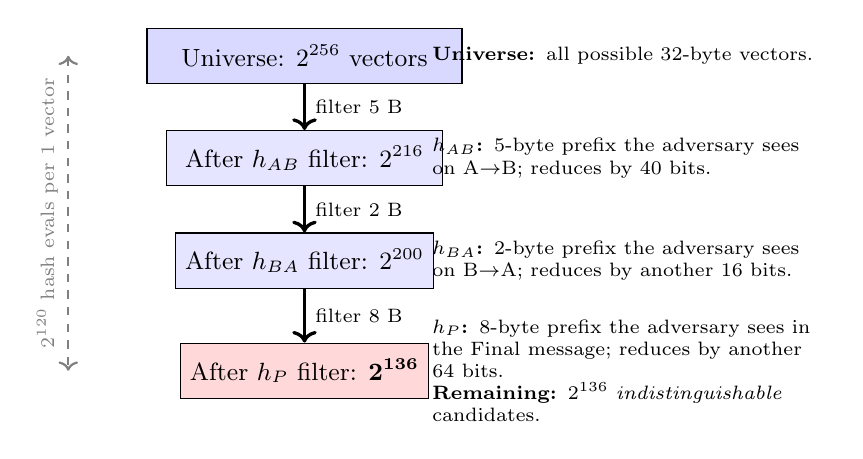
\begin{tikzpicture}[font=\small, scale=1.0]
  % Filter cascade
  \node[draw, fill=blue!15, minimum width=4cm, minimum height=0.7cm] (univ) at (0, 4) {Universe: $2^{256}$ vectors};

  \node[draw, fill=blue!10, minimum width=3.5cm, minimum height=0.7cm] (hab) at (0, 2.7) {After $h_{AB}$ filter: $2^{216}$};
  \draw[->, very thick] (univ) -- node[right, font=\scriptsize] {filter 5 B} (hab);

  \node[draw, fill=blue!10, minimum width=3cm, minimum height=0.7cm] (hba) at (0, 1.4) {After $h_{BA}$ filter: $2^{200}$};
  \draw[->, very thick] (hab) -- node[right, font=\scriptsize] {filter 2 B} (hba);

  \node[draw, fill=red!15, minimum width=2.5cm, minimum height=0.7cm] (hp) at (0, 0.0) {After $h_P$ filter: $\mathbf{2^{136}}$};
  \draw[->, very thick] (hba) -- node[right, font=\scriptsize] {filter 8 B} (hp);

  % Annotation: 2^120 work
  \draw[<->, dashed, thick, gray] (-3, 4) -- node[left, font=\scriptsize, rotate=90, anchor=south] {$2^{120}$ hash evals per 1 vector} (-3, 0);

  % Right side: notes
  \node[font=\scriptsize, anchor=west, text width=5cm] at (1.5, 4) {\textbf{Universe:} all possible 32-byte vectors.};
  \node[font=\scriptsize, anchor=west, text width=5cm] at (1.5, 2.7) {\textbf{$h_{AB}$:} 5-byte prefix the adversary sees on A$\to$B; reduces by 40 bits.};
  \node[font=\scriptsize, anchor=west, text width=5cm] at (1.5, 1.4) {\textbf{$h_{BA}$:} 2-byte prefix the adversary sees on B$\to$A; reduces by another 16 bits.};
  \node[font=\scriptsize, anchor=west, text width=5cm] at (1.5, 0.0) {\textbf{$h_P$:} 8-byte prefix the adversary sees in the Final message; reduces by another 64 bits. \\
  \textbf{Remaining:} $2^{136}$ \emph{indistinguishable} candidates.};

\end{tikzpicture}
\caption{The defense cascade around one password vector. The adversary sees 3 hash prefixes from different phases of the protocol (5 + 2 + 8 B = 15 B = 120 bits). Finding any vector that satisfies all three takes $2^{120}$ hashes. But even such a vector is 1 of $2^{136}$ indistinguishable candidates --- without a validation oracle there is no way to tell which is correct.}
\label{fig:defense-cascade}
\end{figure}

\subsection{Three defenses combined}

A short summary at the end: the three structural defenses of Grata Cascade and how they reinforce one another:

\begin{itemize}[leftmargin=*]
\item \textbf{Drift (Stat) + tail selection} (§\ref{pop:drift}): candidates are \emph{structurally} in the tail, out of reach of direct sampling.
\item \textbf{AES without padding + a short $h_{BA}$} (§\ref{pop:aes}): candidates are \emph{indistinguishable} under flooding, no validation oracle.
\item \textbf{Cumulative preimage barrier} ($\lambda = 120$ bits): a hard lower bound on adversarial work, independent of drift/AES.
\end{itemize}

An adversary aiming for $K^*$ has to bypass \emph{all three} simultaneously. The empirical evaluation (Chapter~\ref{pop:empirical}) shows that none of the 5 evaluated adversary classes achieved any of them on 300 transcripts each.

\section{Empirical evidence}\label{pop:empirical}

So far we have talked about \emph{what the protocol does} and \emph{why it should work}. This chapter shows \emph{what actually happened} when we ran it. These are not theoretical estimates or simulations --- they are real runs of the C\# implementation (.NET 9, post-F3 SHA-NI), reproducible from the repo under \texttt{configs/reference.json} and \texttt{reports/refv2/}.

\begin{tldr}[How to read the tables in this chapter]
Three statistical concepts will recur in the tables. In plain language:
\begin{itemize}[leftmargin=*]
\item \textbf{NIST SP 800-22} is a standard battery of 12 tests that check whether a bit sequence ``looks like random noise''. Each test either passes (PASS) or fails at the configured significance level $\alpha = 0{,}01$. ``12/12 PASS'' means that across 1\,000 keys none of the standard tests detected a deviation from randomness.
\item \textbf{Clopper-Pearson upper 95\% CI} is a conservative statistical ceiling: with $k$ successes out of $n$ trials we want to say ``the population rate is, with 95\% confidence, no higher than this''. For 0/300 the upper bound is $\approx 1{,}22\%$ --- read as ``even at 95\% confidence we cannot claim the failure rate sits below 1{,}22\%''.
\item \textbf{Cohen's $d$} is an effect size: $d \approx 0$ means ``no measurable difference'', $d = 0{,}2$ a small effect, $d = 0{,}5$ medium, $d = 0{,}8$ large. For our discriminator $d = 0{,}009$ sits at the edge of Poisson noise --- comparable to looking at two batches of coin flips.
\end{itemize}
Full definitions are in the glossary, §\ref{pop:glossary}.
\end{tldr}

We will be citing the key numbers repeatedly, so let us collect them up front:

\begin{tldr}[Empirical headline for reference v2]
\begin{itemize}[leftmargin=*]
\item $50\,000$ convergence runs: $99{,}9920\%$ success ($4$ divergences). CP upper 95\% CI: $2{,}05 \times 10^{-4}$.
\item $h_{AB}=6$ ablation ($50\,000$ runs): \textbf{$0$ divergences}. CP upper 95\% CI: $7{,}38 \times 10^{-5}$, below baseline.
\item NIST SP 800-22: $12/12$ PASS over $1\,000$ keys, lowest $p$-value $0{,}3156$.
\item Five classes of passive adversaries (B.1, B.2, B.3, B.4, B.7), $0/300$ recoveries of $K^*$. CP upper per class: $1{,}22\%$.
\item B.4 AES-Oracle discriminator: Cohen's $d = 0{,}009$ over $2{,}05 \times 10^{10}$ queries --- \textbf{no measurable signal}.
\end{itemize}
\end{tldr}

Now let us walk through each experiment and what it means.

\subsection{Convergence: $50\,000$ runs, $4$ divergences}\label{pop:exp-convergence}

Reference v2 was tested on $5 \times 10^4$ independent runs (5 parallel shards of $10\,000$). Each run: an Alice-Bob pair independently initialised, the protocol runs to termination, two binary metrics are evaluated:
\begin{itemize}[leftmargin=*]
\item \textbf{Final-hit (FH)}: did the protocols reach the Final phase (the $\tau$ termination trigger)?
\item \textbf{Keys-match (KM)}: does Alice's $K^*$ match Bob's $K^*$?
\end{itemize}

The results are in Table~\ref{tab:pop-convergence}.

\begin{table}[ht]
\centering
\small
\begin{tabular}{lrr}
\toprule
Outcome & Number of runs & Rate \\
\midrule
$\text{FH}=\text{true} \land \text{KM}=\text{true}$ (success) & $49\,996$ & $99{,}9920\%$ \\
$\text{FH}=\text{true} \land \text{KM}=\text{false}$ (divergence) & $4$ & $0{,}0080\%$ \\
$\text{FH}=\text{false}$ (structural failure) & $0$ & $0{,}0000\%$ \\
\bottomrule
\end{tabular}
\caption{Reference v2 convergence baseline. Per-shard divergence distribution $\{1, 0, 2, 0, 1\}$ is Poisson-consistent with a rate of $\sim 8 \times 10^{-5}$. Iteration distribution: median 49, p95 62, max 90. Median elapsed time: $1{,}71$ s/run.}
\label{tab:pop-convergence}
\end{table}

\textbf{What do divergences mean?} In 4 cases (out of 50 thousand) Alice and Bob both reached termination, but their $K^*$ values did not agree. Structurally this is not catastrophic --- in such a case a higher-level (transport) check detects the key mismatch and the session restarts. But it is a sign that $h_{AB}$ collisions still occasionally slip through (analytically $\sim 8 \times 10^{-5}$, observed $4/50000 = 8 \times 10^{-5}$ --- tight match).

\textbf{What is the upper ceiling?} Clopper--Pearson one-sided upper 95\% CI on the failure rate: $2{,}048 \times 10^{-4}$. That is an explicit statistical ceiling --- with 95\% probability the population rate does not exceed $2 \times 10^{-4}$.

\subsection{Ablation $h_{AB} = 6$: how to push $h_{AB}$ to zero divergences}\label{pop:exp-habresidual}

Reference v2 has $h_{AB} = 5$ B (40 bits). Our model predicts that $h_{AB}$ collisions are the dominant source of residual divergences: 4 divergences out of 50 thousand match the analytic $\mathbb{E}[\text{collisions}] = N^2 / 2^{40} = 4096^2 / 2^{40} \approx 1{,}5 \times 10^{-5}$ per round, $\times 50$ rounds/session $\approx 7{,}5 \times 10^{-4}$, multiplied by $1/M=1/8$ probability of "hitting" a password slot $\approx 9 \times 10^{-5}$ --- in reasonable agreement with the observed $8 \times 10^{-5}$.

Then: increasing $h_{AB}$ from 5 to 6 (adding 8 bits) should reduce the collision rate $256\times$, to $\sim 3 \times 10^{-7}$. Empirical test:

The profile \texttt{reference\_h\_AB6} (a clone of reference v2 with $h_{AB} = 5 \to 6$, all else identical) was run for $5 \times 10^4$ convergence trials.

\begin{table}[ht]
\centering
\small
\begin{tabular}{lrrrrr}
\toprule
\textbf{Profile} & \textbf{$h_{AB}$ (bit)} & \textbf{$N$} & \textbf{$n$} & \textbf{Observed} & \textbf{CP upper 95\% CI} \\
\midrule
F13-v2 IoT             & $32$ & $1024$ & $200$ & $1/200 = 5 \times 10^{-3}$ & $2{,}8 \times 10^{-2}$ \\
Reference v2 (anchor) & $40$ & $4096$ & $50\,000$ & $4/50\,000 = 8 \times 10^{-5}$ & $2{,}05 \times 10^{-4}$ \\
\textbf{$h_{AB}=6$ ablation} & \textbf{$48$} & \textbf{$4096$} & \textbf{$50\,000$} & \textbf{$0/50\,000$} & \textbf{$7{,}38 \times 10^{-5}$} \\
F11-v2 pq128 & $48$ & $8192$ & $200$ & $0/200$ & $1{,}5 \times 10^{-2}$ \\
\bottomrule
\end{tabular}
\caption{$h_{AB}$ residual scaling across 4 empirical points (16-bit $h_{AB}$ span: 32 → 48). The $h_{AB}=6$ row is the cleanest test --- it varies only $h_{AB}$ relative to the baseline, all other parameters fixed. Observed 0 divergences in 50 thousand runs, CP upper 95\% CI \textbf{lies below} reference v2 baseline.}
\label{tab:pop-hab-scaling}
\end{table}

\begin{aha}[Empirical confirmation of the model]
The $h_{AB}=6$ ablation confirms the predictions:
\begin{itemize}[leftmargin=*]
\item Yes, $h_{AB}$ collisions \emph{were} the dominant source. +1 byte removed them.
\item Predicted rate $\sim 3 \times 10^{-7}$; observed upper bound $7{,}38 \times 10^{-5}$ (50k is not enough to distinguish from zero, but it is below baseline).
\item Convergence did not slow down: median iter still 49 (= reference). Bandwidth overhead: +4 KB/round at $N=4096$ ($\sim 20\%$ of the A→B channel).
\end{itemize}

That is why \texttt{reference\_h\_AB6} qualifies as a \textbf{candidate for the v3 reference profile}.
\end{aha}

\subsection{NIST SP 800-22: do the keys look like random noise?}\label{pop:exp-nist}

We collected $1\,000$ independent reference v2 keys ($999$ usable after excluding one KM-divergence) and ran the 12-test NIST SP 800-22 suite on them --- the standard statistical battery for pseudorandom generators. Aggregate bitstream: $255\,744$ bits.

\textbf{Result:} $12/12$ PASS at $\alpha = 0{,}01$. Lowest $p$-value $0{,}3156$ (Binary Matrix Rank --- the most demanding test, and we cleared it with margin). This means: Grata Cascade $K^*$ keys are statistically \emph{indistinguishable from genuinely random sequences} under the broadest standard battery.

\subsection{Calibration sweeps: where it stops working}\label{pop:exp-sweeps}

In Chapter~\ref{pop:drift} we claimed $p_\text{upd} \in [0{,}6, 0{,}95]$ is a narrow operating range. Here is the empirical validation across 3 sweeps.

\paragraph{$p_\text{upd}$ sweep.}
Values $\{0{,}1, 0{,}25, 0{,}5, 0{,}75, 0{,}9, 0{,}95, 1{,}0\}$ with $\theta_\text{cand} = -95$ (filter on):

\begin{table}[ht]
\centering
\small
\begin{tabular}{rrrrrr}
\toprule
$p_\text{upd}$ & FH/N & iter(p50) & Stat entropy & Stat max prob & avg pw $\log_2$ \\
\midrule
$0{,}10$ & 0/50 & 201 (cap) & $7{,}55$ & $0{,}04$ & --- \\
$0{,}25$ & 0/50 & 201 (cap) & $7{,}09$ & $0{,}09$ & --- \\
$0{,}50$ & 0/50 & 201 (cap) & $6{,}13$ & $0{,}16$ & --- \\
\textbf{$0{,}75$} (ref) & \textbf{200/200} & \textbf{67} & $4{,}49$ & $0{,}33$ & $-165{,}10$ \\
$0{,}90$ & 174/200 & 106 & $2{,}69$ & $0{,}58$ & $-167{,}45$ \\
$0{,}95$ & 0/50 & 201 (cap) & $1{,}68$ & $0{,}74$ & --- \\
$1{,}00$ & 0/50 & 201 (cap) & $0{,}00$ & $1{,}00$ & --- \\
\bottomrule
\end{tabular}
\caption{The $p_\text{upd}$ sweep validates the narrow operating range. Below 0{,}5: drift does not form (Stat stays close to uniform, entropy 7{,}55), tail-selection is ineffective. Above 0{,}95: Stat collapses (max-prob approaches 1), tail-selection loses its structure. Sweet spot: $0{,}75$.}
\label{tab:pop-pupd-sweep}
\end{table}

\paragraph{$s$ sweep (seed perturbation).}
We tested $s \in \{1, 2, 3, 5, 7, 10, 15, 30\}$. \textbf{Convergence is invariant} across the entire range: $1600/1600$ successes, median iteration variance $\pm 1$, avg pw log\_2 variance $\pm 1{,}3$ bits. This matters: the pool density $\rho_\text{pool}$ moves by 182 bits (from $-38{,}7$ at $s=1$ to $-220{,}9$ at $s=30$) without affecting convergence. Drift dominates pool density.

While we were at it we also ran a \textbf{re-test of the B.4 AES-Oracle adversary} under dense conditions ($s=1$, $\rho \approx 2^{-38}$ --- 39 bits denser than reference): a null discriminator signal was confirmed across $2{,}3 \times 10^8$ near-seed samples. This empirically refutes the hypothesis that pool density is the defense --- the actual defense is AES key derivation without padding.

\paragraph{$\theta_\text{cand}$ ablation.}
We repeated the $p_\text{upd}$ sweep with the CandMax filter disabled:

\begin{table}[ht]
\centering
\small
\begin{tabular}{rrrr}
\toprule
$p_\text{upd}$ & FH/N (filter $-95$) & FH/N (off) & avg pw $\log_2$ off \\
\midrule
$0{,}75$ & 200/200 & 200/200 & $-158$ \\
$0{,}90$ & 174/200 & 200/200 & $-150$ \\
$0{,}95$ & 0/50 & 200/200 & $-143$ \\
$1{,}00$ & 0/50 & 200/200 & $\boldsymbol{-53}$ \\
\bottomrule
\end{tabular}
\caption{Ablation of $\theta_\text{cand}$'s security role: with the filter off, high $p_\text{upd}$ \emph{preserves convergence} but candidates collapse from $\log_2 \Pr \approx -160$ to $-53$ at $p_\text{upd}=1{,}0$. Those candidates are then in the reconstructible Stat distribution and the adversary can sample them directly. The filter is therefore a structural defense, not just "cleanup".}
\label{tab:pop-cand-ablation}
\end{table}

\subsection{Per-profile validation: does it work outside reference?}\label{pop:exp-profiles}

We validated all 5 profiles separately (200 runs each + 100-key NIST battery):

\begin{table}[ht]
\centering
\small
\begin{tabular}{lrrrrl}
\toprule
Profile & FH/N & KM/N & iter(med) & NIST PASS/N/A & Note \\
\midrule
Reference v2 & 200/200 & 200/200 & 49 & 12/12, 0 N/A & Primary \\
IoT & 200/200 & 200/200 & 68 & 11/12, 1 N/A & $h_P=4$ post-fix \\
Mobile & 200/200 & 200/200 & 48 & 11/12, 1 N/A & --- \\
HighSec Classical & 200/200 & 200/200 & 89 & 11/12, 1 N/A & --- \\
HighSec PQ128 & 50/50 & 50/50 & 69 & 10/12, 1 N/A & 1 marginal Block Freq \\
\bottomrule
\end{tabular}
\caption{Per-profile validation across 5 profiles. "N/A" is Binary Matrix Rank skipped (a 100-key battery yields 25\,600 bits, BMR needs $\geq 38\,912$ bits). HighSec PQ128 has 1 marginal failure (Block Frequency, $p=0{,}0035$) consistent with multi-test battery noise; a disambiguation re-run is planned.}
\label{tab:pop-profiles-validation}
\end{table}

\textbf{Lesson from IoT}: the original IoT config ($h_P = 3$ B = 24 bits preimage) showed $\sim 2{,}5\%$ silent key mismatches (Final hash collisions). Raising it to $h_P = 4$ B (32 bits) fixed it: $200/200$ KM, +8 bits cumulative security, +8 B/Final message. This shows that per-profile calibration is not a luxury --- different scales need different hashes.

\subsection{Five classes of passive adversaries}\label{pop:exp-attackers}

We implemented and evaluated 5 classes of passive adversaries. The first 4 (B.1--B.4) on reference v2 across $N = 300$ transcripts; the fifth (B.7) on the research-only \texttt{break\_demo} (a deliberately weakened config for pedagogical demonstration).

\paragraph{B.1 Baseline Random.} Uniform random sampling, looks for hash matches. Time budget 600 s/transcript. Expected work per slot: $2^{64}$.

\paragraph{B.2 Hash-First Filtered.} Cascading filtration through 3 hashes (A→B 5B, B→A 2B, Final 8B). Filter factor $2^{120}$. Pool $10^7$.

\paragraph{B.3 Tail-Informed Sampler.} A modification of B.2 that draws candidates from the reconstructed Stat tail. Pool $10^7$.

\paragraph{B.4 AES-Oracle Discriminator.} For a hypothetical stage-b candidate, decrypts AES, regenerates the near-seed pool, and validates against the next round's hashes. Measures discriminator power (TP/FP rates, Cohen's $d$). $K = 10^6$ samples per round-pair.

\paragraph{B.7 Stat-Sorted Enumeration.} Instead of random sampling, B.7 \emph{deterministically orders} vectors by their probability under $\mathcal{S}$ and walks them in that order (from most likely down, or from least likely up). Implemented with a priority queue --- it aims squarely at the peaks or the slivers of the wheel of fortune, never at a random sector. Two modes:
\begin{itemize}[leftmargin=*]
\item \emph{Typical}: vectors in decreasing Stat probability (typical bytes); designed to match A's pool.
\item \emph{Tail}: vectors in increasing Stat probability (rare bytes); designed to match the protocol's CandMax-filtered password set.
\end{itemize}
Validation on \texttt{break\_demo} ($\lambda_\text{preimage}=56$ bits, parameters deliberately weakened so that an attack is theoretically close to feasible but still slightly above the breaking threshold): $0/300$ key recoveries in either mode. The dual-mode behaviour shows that the cascade blocks Stat-prior enumeration in \emph{either} direction.

\paragraph{Main results.}

\begin{table}[ht]
\centering
\small
\begin{tabular}{lrrrrr}
\toprule
Adversary & Runs & $K^*$ recovery & Success rate & 95\% CI upper & Avg time/run \\
\midrule
B.1 Baseline Random & 300 & 0 & $0{,}000\%$ & $1{,}222\%$ & $600{,}0$ s (cap) \\
B.2 Hash-First & 300 & 0 & $0{,}000\%$ & $1{,}222\%$ & $56{,}7$ s \\
B.3 Tail Sampler & 300 & 0 & $0{,}000\%$ & $1{,}222\%$ & $130{,}5$ s \\
B.4 AES-Oracle & 300 & 0 & $0{,}000\%$ & $1{,}222\%$ & $335{,}1$ s \\
B.7 Stat-Sort. Tail (on \texttt{break\_demo}) & 300 & 0 & $0{,}000\%$ & $1{,}222\%$ & $59{,}0$ s ($10^7$ pool) \\
\bottomrule
\end{tabular}
\caption{Passive-adversary evaluation. B.1--B.4 under reference v2 across $N=300$ transcripts (shared set). Total compute $\sim 10^{11}$ SHA-256 evaluations, wall-clock 6h 33m on 22 workers. B.7 reports the \texttt{break\_demo} dual-mode evaluation (Tail mode at $10^7$ pool); evaluation of B.7 against reference v2 is deferred.}
\label{tab:pop-attackers}
\end{table}

\textbf{B.4 Cohen's $d = 0{,}009$}: across 10\,262 round-pairs and $2{,}05 \times 10^{10}$ queries, mean TP $0{,}003411$, mean FP $0{,}002923$. The empirical FP is in the predicted SHA-oracle band ($\mathbb{E}[\text{FP}] = 0{,}003725$). \textbf{No measurable discriminator signal.}

\textbf{Stage cascade validation (B.2)}: across 300 transcripts, 503 rounds with stage-a hits ($515$ hits in total), $0$ stage-b, $0$ stage-c. Stage-a hits match the analytic cascade within Poisson noise. The filter behaves as designed.

\subsection{Visualisation: adversary effectiveness vs random baseline}

\begin{figure}[h]
\centering
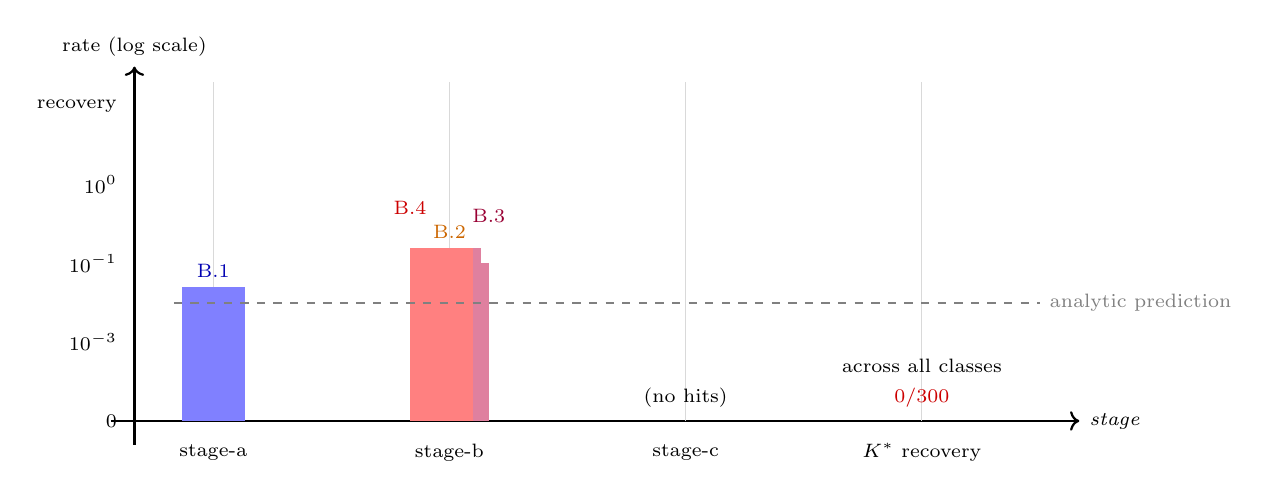
\begin{tikzpicture}[font=\small, scale=1.0]
  % Axes
  \draw[->, thick] (-0.3, 0) -- (12, 0) node[right, font=\scriptsize] {\textit{stage}};
  \draw[->, thick] (0, -0.3) -- (0, 4.5) node[above, font=\scriptsize] {rate (log scale)};

  % X labels for stages
  \foreach \x/\lab in {1/{stage-a}, 4/{stage-b}, 7/{stage-c}, 10/{$K^*$ recovery}} {
    \node[font=\scriptsize] at (\x, -0.4) {\lab};
    \draw[gray!30] (\x, 0) -- (\x, 4.3);
  }

  % Y labels log scale
  \foreach \y/\lab in {0/0, 1/{$10^{-3}$}, 2/{$10^{-1}$}, 3/{$10^0$}, 4/recovery} {
    \node[font=\scriptsize, anchor=east] at (-0.1, \y) {\lab};
  }

  % B.1 random: stage-a baseline
  \fill[blue!50] (0.6, 0) rectangle (1.4, 1.7);
  \node[font=\scriptsize, blue!70!black] at (1, 1.9) {B.1};

  % B.2 hash-first
  \fill[orange!60] (3.6, 0) rectangle (4.4, 2.2);
  \node[font=\scriptsize, orange!80!black] at (4, 2.4) {B.2};

  % B.3 tail
  \fill[purple!50] (3.6, 0) rectangle (4.4, 2.2);
  \fill[purple!50] (3.7, 0) rectangle (4.5, 2.0);
  \node[font=\scriptsize, purple!80!black] at (4.5, 2.6) {B.3};

  % B.4 AES Oracle
  \fill[red!50] (3.5, 0) rectangle (4.3, 2.2);
  \node[font=\scriptsize, red!80!black] at (3.5, 2.7) {B.4};

  % stage-c: no hits
  \node[font=\scriptsize] at (7, 0.3) {(no hits)};

  % K* recovery: zero
  \node[font=\scriptsize, text=red!80!black] at (10, 0.3) {0/300};
  \node[font=\scriptsize] at (10, 0.7) {across all classes};

  % Overlay: predicted random rate
  \draw[dashed, thick, gray] (0.5, 1.5) -- (11.5, 1.5);
  \node[font=\scriptsize, gray, anchor=west] at (11.5, 1.5) {analytic prediction};

\end{tikzpicture}
\caption{Schematic view of adversary effectiveness (B.1--B.4) across the cascade. Stage-a: every adversary gets hits consistent with the analytic prediction (Poisson noise around the dashed line). Stage-b: 0 hits --- the combined $h_{AB} + h_{BA}$ filter (56 bits) stops them all. Stage-c and $K^*$ recovery: zero. No adversary recovered $K^*$ from 300 transcripts.}
\label{fig:attacker-effectiveness}
\end{figure}

\subsection{What the experiments together say}

\begin{tldr}[Summary of empirical evaluation]
\begin{itemize}[leftmargin=*]
\item The protocol \textbf{almost always converges} (99{,}992\% or better over 50k runs).
\item The output keys look \textbf{statistically random} (NIST 12/12 PASS).
\item The parameter operating ranges are \textbf{empirically delimited} and enforced at config load.
\item None of the 5 adversary classes (classified strategies + budget $\sim 10^{11}$ SHA evaluations) \textbf{recovered $K^*$}.
\item B.4 AES-Oracle, the most sophisticated discriminator-based attack, has \textbf{Cohen's $d = 0{,}009$} --- the kind of TPM-style gradient-leak attack did not just fail to "win" --- it failed to be \emph{measurable at all}.
\item The $h_{AB}=6$ ablation shows that strengthening $\lambda$ to 128 bits is \textbf{empirically free} (median iter unchanged, +4 KB/round bandwidth).
\end{itemize}
\end{tldr}

This is not a formal proof that the protocol is unbreakable. It is strong empirical evidence that \emph{within the tested range} it behaves as advertised. What remains open (ML adversaries, multi-round aggregation, formal reduction) we will go through in Chapter~\ref{pop:open}.

\section{Comparison with one-shot KE primitives}\label{pop:comparison}

\noindent\textit{What to take away: Grata Cascade is roughly 3 orders of magnitude worse on bandwidth than ML-KEM (the post-quantum standard) and almost 5 orders worse than ECDH (the classical standard). Its potential value is not efficiency but \emph{structural cryptographic diversification}: it rests on a third independent base (hash preimage + drift), so in an X-Wing-style hybrid stack it adds a third coequal layer whose simultaneous breakage with DLP \emph{and} lattices would require three independent cryptanalytic advances.}

\medskip

In this booklet and in the paper Grata Cascade is positioned as a \emph{one-shot} key agreement primitive. The comparison therefore targets existing one-shot KE primitives (ECDH, ML-KEM, X-Wing hybrid, Merkle puzzles), not continuous key agreement (CKA) constructions like Signal Double Ratchet, MLS, or Triple Ratchet --- the relation to CKA is described in Chapter~\ref{pop:open} (\texttt{prob:cka-extension}).

\begin{table}[ht]
\centering
\small
\begin{tabular}{lllll}
\toprule
Scheme & Base & PQ security & Bandwidth / session & Formal proof \\
\midrule
ECDH (X25519) & DLP & No (Shor) & $\sim 32$ B & Yes (ROM) \\
ML-KEM-768 & Module-LWE & Yes & $\sim 1{,}2$ KB & Yes (ROM) \\
X-Wing & DLP $+$ Module-LWE & Yes & $\sim 1{,}3$ KB & Yes \\
Merkle puzzles (1978) & Hash preimage & Yes (Grover) & $O(N^2)$ work & Yes (IR89) \\
\textbf{Grata Cascade ref v2} & Hash preimage $+$ drift & Yes (conj.) & $\sim 1$ MB & No (open) \\
\bottomrule
\end{tabular}
\caption{Comparison of one-shot KE primitives. ``Conj.'' = conjectural (structurally argued, not formally proved). ``IR89'' = Impagliazzo--Rudich black-box bound. Bandwidth for ECDH and ML-KEM is round-trip; for Grata Cascade it is per session ($\sim 49$ rounds $\times$ $\sim 20$ KB).}
\label{tab:pop-comparison}
\end{table}

Grata Cascade is in transmitted bandwidth \emph{about three orders of magnitude worse} than ML-KEM ($\sim 1{,}2$ KB) and almost five orders worse than ECDH ($\sim 32$ B). That is a fundamental engineering disadvantage and rules it out for the vast majority of production deployments where bandwidth is a sensitive parameter (mobile data, IoT). Optimisation paths are open in~\texttt{prob:bandwidth} (Chapter~\ref{pop:open}).

So why would anyone want it?

\subsection{The value: a third independent layer in a hybrid composition}

The current NIST-recommended X-Wing hybrid combines X25519 (ECDH) with ML-KEM-768. An adversary must break \emph{both} bases to recover the key:

\begin{itemize}[leftmargin=*]
\item \textbf{DLP} broken by a quantum computer (Shor, expected). X25519 falls but ML-KEM holds.
\item \textbf{Module-LWE} broken by an unexpected attack. Lattice cryptography is relatively young (NIST standardisation 2024); if someone finds a polynomial algorithm, ML-KEM falls. Then X25519 holds (against pre-quantum attackers) but not against an attacker with a quantum computer.
\item \textbf{Both at once} (quantum computer $+$ lattice break): X-Wing falls. No fallback.
\end{itemize}

Grata Cascade can add a \textbf{third independent layer} to the hybrid stack, resting on an entirely different principle than DLP or lattices:

\begin{itemize}[leftmargin=*]
\item \textbf{Base: hash preimage + statistical drift.} Does not depend on DLP nor on lattice problems. Hash functions are a structurally different type of cryptographic primitive than algebraic constructions.
\item \textbf{Long battle-testing.} SHA-256 has existed since 2001 and is deployed across virtually every cryptographic context (TLS, signatures, code commitments). Attacks against hashes have been intensely researched for decades.
\item \textbf{Solid post-quantum security.} Grover's algorithm speeds up preimage by $\sqrt{}$, so the full SHA-256 stays post-quantum-secure at $2^{128}$. Our cumulative barrier $\lambda = 120$ bits is therefore post-quantum $2^{60}$ --- at the edge of the weaker threshold; the v3 candidate \texttt{reference\_h\_AB6} pushes it to $\lambda = 128$ bits, post-Grover $2^{64}$.
\end{itemize}

\begin{aha}[Diversification, not replacement]
Grata Cascade is \emph{not} an attempt to replace ECDH or ML-KEM. Those are markedly more efficient (roughly $1\,000\times$ to $100\,000\times$ smaller bandwidth) and carry formal proofs. The goal of Grata Cascade: be a \emph{third coequal layer} in the hybrid stack --- concretely an extended X-Wing-style: X25519 $\oplus$ ML-KEM-768 $\oplus$ Grata Cascade. If an attacker breaks two of these three bases (e.g.\ a quantum computer $+$ a lattice break), Grata Cascade as the third still holds. If Grata Cascade fell, X-Wing still holds against that attacker. The value is in the \emph{independence} of bases, not performance.
\end{aha}

\subsection{Versus Merkle puzzles}

The classical hash-based KE primitive, Merkle puzzles (1978), achieves $O(N^2)$ adversarial work over $O(N)$ legitimate work. By Impagliazzo--Rudich (1989) this is the optimum in the black-box model: no construction purely on top of a one-way function reaches better than quadratic security. For $\lambda = 128$ bits this requires $N \approx 2^{64}$ puzzles, which is deployment-prohibitive bandwidth (on the order of exabytes).

Grata Cascade conjecturally beats this black-box bound through the combination of a hash with statistical drift. If formally confirmed (open problem~\texttt{prob:dynamic-formal}), this would be the first deployable hash-only KE primitive with a better bandwidth-security trade-off than Merkle. But even without a formal reduction Grata Cascade is already $\sim 3$ orders of magnitude better than Merkle in the $\lambda = 120$-bit regime ($\sim 1$ MB session vs.\ exabytes).

\subsection{What Grata Cascade lacks}

Let us be honest: beyond bandwidth the protocol has further weaknesses.

\begin{itemize}[leftmargin=*]
\item \textbf{No formal proof.} ECDH and ML-KEM have \emph{game-based} security reductions in the random-oracle model (ROM) to the hardness of their underlying problems; the reductions are peer-reviewed and standardised. Grata Cascade, by contrast, has only \emph{structural arguments} and \emph{empirical validation} for a passive adversary. The open problem \texttt{prob:dynamic-formal} (§\ref{pop:open}) sketches an analogous reduction, but it is not done --- the gap between ``structurally compelling'' and ``formally proved'' remains.
\item \textbf{Higher compute cost.} $\sim 1{,}71$ s per convergence on a desktop CPU, vs.\ milliseconds for an ECDH update. For IoT/battery, that matters.
\item \textbf{Parametric profiles not fully evaluated.} Mobile and HighSec are calibrated but lack a per-profile adversary evaluation at $N = 300$ transcripts (open problem \texttt{prob:parametric}).
\item \textbf{Not a CKA.} Grata Cascade produces \emph{one} key $K^*$ per session; it does not cover the inter-message rotation that the Triple Ratchet provides in the Signal stack. Extending to a CKA primitive is a separate open direction (\texttt{prob:cka-extension}).
\item \textbf{Unstable against active adversaries.} Without an authenticated transport (TLS, Noise) an active adversary can modify $R_t$ and degrade the protocol. Three optional defenses (statistical detection, deterministic $R_t$, public $R$-pool) are sketched in the v9 main appendix, but not field-tested.
\end{itemize}

We do not sweep this under the rug --- in Chapter~\ref{pop:open} we walk through these open problems in more detail.

\section{What we still do not know: open problems}\label{pop:open}

No research is finished. This chapter is an honest list of questions that we do not have an answer to yet. Some are \emph{central} (a solution would change our perspective fundamentally), some are \emph{engineering} (their solution would make the protocol more practical), some are \emph{extensions} (interesting but not necessary for the core claims).

\subsection{Central problems}

\paragraph{prob:cka-extension --- Extension to a CKA primitive.} Grata Cascade in this work is a \emph{one-shot} primitive: one session, one key $K^*$, done. Full integration into a Signal-style messaging stack requires \emph{continuous key agreement} (CKA): a protocol producing a sequence of keys $\{k_1, k_2, k_3, \ldots\}$ across the conversation with formal forward secrecy and post-compromise security guarantees. We sketch three possible paths:

\begin{itemize}[leftmargin=*]
\item \textbf{Path A --- Repeated-session chaining (primary target).} Run GC repeatedly, with each new session using the previous $K^*$ as a seed plus fresh randomness. Expensive ($\sim 1$ MB per rotation), but a clean reduction to single-session security. The main target for a follow-up paper with a formal reduction.
\item \textbf{Path B --- Symmetric ratchet on top of a GC bootstrap.} Use GC to derive $K^*_0$, then $K^*_i = \mathrm{HKDF}(K^*_{i-1}, \mathrm{salt}_i)$ as in Signal's symmetric KDF ratchet. Cheap and immediately deployable, but PCS is inherited only from the bootstrap, not from the ratchet itself.
\item \textbf{Path C --- Native CKA construction.} Redesign GC so that each round emits a \emph{released} key plus a \emph{kept} state (the drift continues). The most novel option, but requires a fundamental redesign and a new security analysis --- a long-term moonshot.
\end{itemize}

\textbf{Why it is central:} without a CKA variant Grata Cascade does not cover the ``one key per message'' use case (Signal). Path A is the most defensible follow-up paper and the logical continuation after \texttt{prob:dynamic-formal} is resolved.

\paragraph{prob:dynamic-formal --- Formalisation of dynamic asymmetry.} The static asymmetry $R \approx n/k$ (Chapter~\ref{pop:static}) gives a \emph{lower bound} on the adversary's disadvantage for a single session. The dynamic mechanisms (drift, hash addressing, multi-round refinement) strengthen that bound --- but by how much and under what conditions? Goal: derive an analytic bound on the adversary's advantage as a function of (number of rounds, parameters, Stat concentration) under a random-oracle model for SHA-256. A reduction to SHA-256 preimage hardness is a sub-component.

\textbf{Why it is central:} solving this problem would convert the empirical security claim ("nobody broke it across 300 transcripts") into a formal cryptographic guarantee ("the adversary's advantage is $\leq 2^{-\lambda}$ for ..."). Without it, Grata Cascade is structurally compelling but lacks a hard mathematical anchor for single-session security. Solving it also provides the basis for Path A in \texttt{prob:cka-extension}.

\subsection{Empirical extensions}

\paragraph{prob:parametric --- Full parametric adversary analysis.} The three production profiles (reference, Mobile, HighSec) are calibrated, but only reference v2 has a per-profile adversary evaluation across 5 classes. Cover Mobile and HighSec with $N \geq 300$ transcripts each. Also: build the Pareto frontier in (security, bandwidth, convergence, memory) space.

\paragraph{prob:multiround --- Multi-round aggregation of weak signals.} The per-round B.4 discriminator has a detection power of $d = 0{,}009$, unmeasurable. An adversary aggregating across $k$ rounds gets effect $d_0 \sqrt{k}$. For $d_0 = 0{,}1$, $k = 50$: $d \approx 0{,}7$, detectable. The question: is such aggregation reachable for adversaries against Grata Cascade --- given that the single-round signal is below the detection threshold?

\paragraph{prob:nist-strong --- Strengthened NIST evaluation at $10^6$ keys.} The current NIST battery uses $1\,000$ keys. With $\geq 10^6$ keys plus a second-order analysis (chi-square uniformity check on the resulting $p$-value distribution) the statistical-uniformity claim would have higher confidence. Doable inside the existing framework, $\sim 1$ day of compute.

\subsection{New adversary classes}

\paragraph{prob:ml --- ML-based adversaries.} Train a deep neural model on the mapping (transcript $\to$ bits of $K^*$). Better than $50\%$? If yes, quantify the leak and identify which transcript features carry signal. A structurally distinct class from B.1--B.7 and not addressed by the current empirical bounds.

\subsection{Engineering optimisation}

\paragraph{prob:bandwidth --- Bandwidth optimisation.} Reference requires $\sim 20$ KB/round, dominated by $N$ hash prefixes on the A→B channel. Could Bloom filters, chunking, or amortisation across rounds bring this below $5$ KB while preserving security? Primarily an engineering effort, but with a large impact on deployment viability.

\paragraph{prob:flood-stress --- Stress-testing the flooding defense at large pools.} The current adversary battery (§\ref{pop:exp-attackers}) evaluates B.1--B.4 at $P = 10^7$. At this pool size the expected number of stage-b survivors is $\approx 4{.}5 \cdot 10^{-6}$ per round (formula $E = P \cdot N \cdot M / 2^{56}$). The $0/300$ outcome therefore means more like ``nobody even reached stage-b'' than ``stage-b worked as a filter against real flooding''. To empirically validate the AES NoPadding defense under genuine pressure we need $P \geq 10^{10}$:

\begin{itemize}[leftmargin=*]
\item \textbf{Prediction at $P = 10^{12}$}: $\approx 22$ stage-b survivors per session (50 rounds), $\approx 1{.}2 \cdot 10^{-18}$ stage-c survivors, $\approx 0$ key recoveries. Measuring would validate the flooding defense under load: the observed stage-b/stage-c hit counts can be compared with the analytic prediction, and in particular we would verify that out of dozens of stage-b candidates per session \emph{none} survives to stage-c (or only as Poisson noise).
\item \textbf{Memory budget:} constant. The pool is streamed (not generated at once); only $\sim$ KB of transcript hashes need to be held. 16 GB of GPU RAM is more than enough.
\item \textbf{Compute budget:}
\begin{itemize}[leftmargin=*]
\item B.2 (pure SHA filtering): the current $P = 10^7$ takes $\approx 57$ s/session. Linear scaling gives $\approx 900$ days for $P = 10^{12} \times 300$ sessions on a 22-core CPU --- prohibitive. On a GPU (RTX 4060/4090 at $5$--$10$ GH/s SHA-256) this drops to \textbf{8--16 hours for the full 300-session batch}.
\item B.4 (AES Oracle): AES decryption on a GPU is orders of magnitude slower than SHA-256, so $P = 10^{12} \times 300$ remains a multi-day-to-week run even on GPU. Practical reduction: $N = 30$ sessions or $P = 10^{10}$.
\end{itemize}
\item \textbf{Plan}: after receiving a dedicated RTX 4060 (around 2026-05-13) run B.2 @ $P \in \{10^{10}, 10^{12}\} \times 300$ sessions and B.4 @ $P = 10^{10} \times 30$ sessions. Extend Table~\ref{tab:pop-attackers} with a new column/rows and compare against the analytic prediction.
\end{itemize}

\paragraph{prob:pupd-dynamic --- Dynamic $p_\text{upd}$.} The static $p_\text{upd} = 0{,}75$ is the empirically calibrated optimum. A dynamic variant where $p_\text{upd}$ is derived from the shared secret state would force the adversary to reconstruct an entire Stat family $\mathcal{S}_\theta$ for an unknown $\theta$, potentially adding bits of effective security. Security gain and convergence implications open.

\subsection{Research parametric families}

\paragraph{prob:iot --- IoT parametric family.} Full calibration of a low-resource profile ($L = 16$, $N \sim 1024$). The indistinguishable-set size at these parameters is only $2^{48}$ --- within reach of brute-force enumeration on modern GPUs. Full calibration under the three-rationale design plus an adversary evaluation are open.

\paragraph{prob:pq128 --- 128-bit post-quantum family.} Design and empirical validation of a profile achieving $128$-bit PQ security under Grover's speedup. Key design question: is PQ security primarily reached via $\lambda_\text{preimage} \geq 256$ (the bandwidth-conservative path) or via structural arguments combining the indistinguishable set + Stat correlation (more elegant, but contingent on solving \texttt{prob:dynamic-formal}).

\subsection{What is, on the contrary, \emph{closed}}

\paragraph{prob:hab-residual --- $h_{AB}$ residual divergence elimination \textbf{[closed in v8]}.} An open problem in earlier paper versions. Closed in v8 by a direct ablation: $h_{AB} = 6$ at reference scale across $5 \times 10^4$ runs gave $0$ KM divergences, CP upper 95\% CI $7{,}38 \times 10^{-5}$, below the reference v2 baseline $8{,}0 \times 10^{-5}$. Full report in §\ref{pop:exp-habresidual}.

\paragraph{prob:breakdemo --- Break-Demo parametric subfamily \textbf{[empirically validated in v8]}.} An open problem in earlier paper versions. In v8 reduced to a pedagogical demonstration: parameters $L = 8, N = 256, h_{AB} = 3, \lambda_\text{preimage} = 56$ bits --- deliberately weakened so the attack would be theoretically close to feasible while still slightly above the breaking threshold. An empirical pilot under the 5-class adversary battery: $0/300$ across all classes. Shown: the cascaded filter blocks Stat-prior enumeration in both directions --- the open question is reachable only at $\lambda \leq 48$ or with adversary classes outside the cascade-filter framework.

\begin{aha}[Honest about scope]
Seven open problems is not a sign that the protocol is "unfinished". It is a sign that we \emph{choose generously}: any time we have a claim, we also have a question about how to improve or refute it. This density of open problems is itself a security feature --- it is a transparent stance of "we do not know this", not "we know everything".
\end{aha}

\section{Glossary and where to go next}\label{pop:glossary}

\subsection{Glossary of terms}

Key terms in popular translation. For the full technical definition see \texttt{docs/glossary.md} (in the repo) or paper v9 main.

\begin{description}[leftmargin=*, style=nextline]
\item[CKA (Continuous Key Agreement)] Continuous key agreement. A messaging mechanism where keys gradually rotate (as the conversation progresses), so that compromise of a single state does not endanger the others.
\item[Ratchet] In secure-messaging cryptography, a mechanism that \emph{progressively rotates the key forward, never backward} (like the pawl on a wrench). An attacker who briefly captures the current key cannot decrypt past messages nor derive future ones. \emph{Triple Ratchet} = three independent ratchets layered in Signal (DH + KEM + symmetric KDF). Grata Cascade in its current form is \emph{not} a ratchet (it produces one key per session); extending it to a CKA primitive with a sequence of keys is the topic of Chapter~\ref{pop:open}, \texttt{prob:cka-extension}.
\item[Forward Secrecy (FS)] A property: today's key compromise does not allow decryption of \emph{past} messages. (If you are exposed tomorrow, today's message is safe.)
\item[Post-Compromise Security (PCS)] A property: after a compromise the protocol gradually "heals" --- new keys generated after the incident are safe even if the adversary briefly saw the internal state.
\item[Diffie-Hellman (DH, ECDH)] Classical key exchange, $g^x$ and $g^y$ are exchanged, the shared key is $g^{xy}$. Broken by Shor's algorithm on a quantum computer.
\item[ML-KEM] Module-Lattice based Key Encapsulation Mechanism. Post-quantum key exchange standardised by NIST in 2024. Triple Ratchet uses it as the second layer.
\item[KEM] Key Encapsulation Mechanism. The broader class of post-quantum primitives that includes ML-KEM (essentially asymmetric encryption used for key exchange).
\item[SHA-256] The standard hash function. One-way: from input the hash is easy, the inverse is intractable. Post-Grover security $2^{128}$.
\item[Preimage resistance] A property of a hash: given a hash value $h$, it is hard to find $v$ such that $H(v) = h$. For SHA-256: $2^{256}$ classically, $2^{128}$ post-Grover.
\item[$\lambda_\text{preimage}$] The cumulative preimage barrier. How many bits of hash constraint the adversary has to overcome per password vector. In reference v2: 120 bits.
\item[$h_{AB}, h_{BA}, h_P$] The three hash prefix lengths (A→B, B→A, password). In ref v2: 5, 2, 8 bytes. Their sum $\times 8$ = $\lambda_\text{preimage}$ = 120 bits.
\item[$\mathcal{V}_A, \mathcal{V}_B$] The private vector pools of Alice and Bob, respectively. In ref v2 each holds 4096 vectors of 32 bytes.
\item[$\mathcal{S}$ (Stat)] The statistical distribution shared between A, B (and the adversary). For each position $i$ a probability vector over the 256 byte values. Updated each round from the public $R_t$.
\item[$R_t$] The public random vector in round $t$. Sent B$\to$A, used as input to the Stat update.
\item[$p_\text{upd}$] Probability that a given vector updates in a given round. In ref v2: 0{,}75. The operating range $[0{,}6, 0{,}95]$ is enforced.
\item[$M$] Number of password candidates per round. In ref v2: 8.
\item[$K^*$] The final shared key, the protocol's output. 32 bytes, usable as an AES-256 key.
\item[Tail selection / CandMax filter] Bob picks candidates with the \emph{lowest} probability under Stat (not the typical ones). A structural defense against direct sampling by the adversary.
\item[NoPadding (PaddingMode.None)] AES mode without padding. Key property: a wrong-key decryption produces pseudo-random bytes (rather than an explicit error) $\Rightarrow$ no validation oracle for the adversary.
\item[Stage-a / stage-b / stage-c] Successive phases of adversary filtering. Stage-a: matches $h_{AB}$. Stage-b: matches $h_{AB} + h_{BA}$. Stage-c: matches $h_{AB} + h_{BA} + h_P$.
\item[FH (Final-Hit)] A binary metric: did the protocol reach the Final phase (termination)?
\item[KM (Keys-Match)] A binary metric: do Alice's and Bob's $K^*$ agree?
\item[Clopper-Pearson CI] A standard statistical upper/lower interval on a binomial rate estimate (successes / n). Conservative, suited to low rates (e.g.\ 0/300).
\item[Cohen's $d$] A standard effect-size metric: $d = (\mu_1 - \mu_2)/\sigma$. $d = 0{,}2$ a small effect, $d = 0{,}5$ medium, $d = 0{,}8$ large. $d = 0{,}009$ is in the Poisson-noise regime.
\item[Conjectural] In a cryptographic context this labels a claim that is structurally well-argued (often supported by empirical evidence) but not yet proved formally. Not ``a hunch'' in the colloquial sense --- in mathematics a conjecture is a precisely formulated proposition whose truth value is open.
\item[Reference v2] The current production parameter baseline (after the 2026-05-02 pivot). $L=32$, $N=4096$, $h_{AB}=5$, $h_{BA}=2$, $h_P=8$, $M=8$, $p_\text{upd}=0{,}75$, $\lambda=120$ bits.
\item[\texttt{reference\_h\_AB6}] A v3 reference candidate. Clone of reference v2 with $h_{AB} = 6$, $\lambda = 128$ bits, +4 KB/round bandwidth.
\item[\texttt{break\_demo}] A deliberately weakened research-only config. $L=8$, $\lambda = 56$ bits --- parameters sit just above the threshold where an attack would theoretically succeed. For pedagogical attack demos, NOT for production.
\end{description}

\subsection{Where to go next}

\paragraph{If you want the full mathematics.} The main paper v9: \texttt{paper/v9/files/paper\_v9\_cz.tex} (CZ) and \texttt{paper\_v9\_en.tex} (EN). Full proofs, formal definitions, complete tables of empirical results, bibliography. Approximately 1180 lines of LaTeX, $\sim 30$ PDF pages.

\paragraph{If you want to reproduce the empirics.} \texttt{docs/REPRODUCE\_PAPER.md}: step-by-step instructions for reproducing the main empirical claims. Three levels:
\begin{itemize}[leftmargin=*]
\item Lv0 sanity ($\sim 30$ s): a simple run, check that the implementation works.
\item Lv1 small ($\sim 10$ min): mini-convergence + small NIST battery.
\item Lv2-3 ($\sim 1$--$24$ h): full validation of 50k runs + NIST $1\,000$ keys + 5 adversary classes on 300 transcripts.
\end{itemize}

\paragraph{If you want the code.} GitHub: \texttt{GrataLuma/Cascade}. Implementation in C\# (.NET 9). Reference v2 in \texttt{configs/reference.json}. Core crypto in \texttt{GrataCascade.Core/}. CLI in \texttt{src/Program.cs}. Reporting in \texttt{Reports/}.

\paragraph{If you want the complete glossary.} \texttt{docs/glossary.md} (289 lines): symbols, parameters, F-task index (F1--F13), profiles, statistical conventions, configuration.

\paragraph{If you want to contribute.} The open problems from Chapter~\ref{pop:open}, prioritised approximately:
\begin{itemize}[leftmargin=*]
\item \textbf{CKA extension} (\texttt{prob:cka-extension}) --- the most important follow-up direction; a concrete research programme along three paths (A: repeated-session chaining, B: symmetric ratchet on top of GC, C: native CKA).
\item \textbf{Formal reduction} (\texttt{prob:dynamic-formal}) --- second central problem; the basis for Path A in the CKA extension.
\item \textbf{Flooding stress test} (\texttt{prob:flood-stress}) --- empirical validation of the AES NoPadding defense at $P = 10^{12}$, GPU-friendly ($\sim 8$--$16$ hours on an RTX 4060).
\item \textbf{ML adversaries} (\texttt{prob:ml}) --- a new class, open ground.
\item \textbf{Bandwidth optimisation} (\texttt{prob:bandwidth}) --- engineering, but high impact.
\item \textbf{Per-profile adversary evaluation} (\texttt{prob:parametric}) --- mechanical, but necessary.
\end{itemize}

\bigskip

\noindent\textit{Thank you for reading this far. If anything in this booklet was unclear, or any claim seems disputable, please open an issue in the repo --- we want the popular version to be genuinely understandable.}

\medskip
\noindent\emph{Birthday paradox describes a static state. Grata Cascade builds a dynamic one-shot system on top of it. The continuous (CKA) variant remains open. And we hope this dynamic, by now, has convinced you.}

\end{document}
